\chapter{GLADE+ Bright Galaxies as Redshift Tracers}
\label{chap:methodology}

The core idea investigated in this thesis is the use of \textbf{bright galaxies} as redshift tracers for \ac{GW} events. The \texttt{GLADE+} galaxy catalog is a comprehensive database of galaxies in the local universe, but it suffers from incompleteness at high redshifts. This incompleteness arises from the limited depth of the catalog, which is primarily designed to cover the local universe, owing to the sensitivity constraints of the current \ac{EM} telescope. We overcome this limitation by focusing on the brightest galaxies in the catalog, which are more likely to be well-represented and can provide a more accurate estimate of the redshift of \ac{GW} events. This essentiaally makes the catalog deeper and more complete at high redshifts, while allowing us to use the \texttt{GLADE+} catalog as a proxy for the underlying matter distribution in the universe.


\section{Bright Galaxy Subsets}
The analysis begins with the construction of \textbf{bright galaxy subsets}, denoted \texttt{GLADEPXX}, where only the top $XX\%$ of galaxies by cumulative $K$-band luminosity are included. The $K$-band luminosity is chosen as it is better associated with the mass of the galaxies \citep{strazzullo2006near,sureshkumar2021galaxy}. Limiting the analysis to these bright subsets allows us to:
\vspace{-1em}
\begin{itemize}
  \item Reduce the out-of-catalog correction by focusing on galaxies likely to be well-represented.
  \vspace{-1em}
  \item Improve the signal-to-noise ratio of the statistical redshift prior.
  \vspace{-1em}
  \item Minimize the inclusion of poorly characterized or faint galaxies.
\end{itemize}

The bright galaxy subsets are defined by selecting galaxies based on their absolute magnitude, which is inferred from their redshift and apparent magnitude. For a given subset, the dimmest galaxy sets the absolute magnitude limit, $M_{max}$, for that subset. This limit is then used in the Schechter luminosity function to adjust the out-of-catalog contribution, effectively reducing its impact. By focusing on the brightest galaxies, we assume that they trace the mass distribution in the Universe more effectively, and are more likely to host \ac{CBC} events.

This approach improves the completeness of the galaxy catalog in the high-redshift regime, as the out-of-catalog contribution becomes smaller. Figure~\ref{fig:z_dist} illustrates how the redshift distribution shift towards higher values making the catalog more complete, highlighting the effectiveness of this method in probing deeper $z$--ranges.

\begin{figure}[h!]
  \centering
  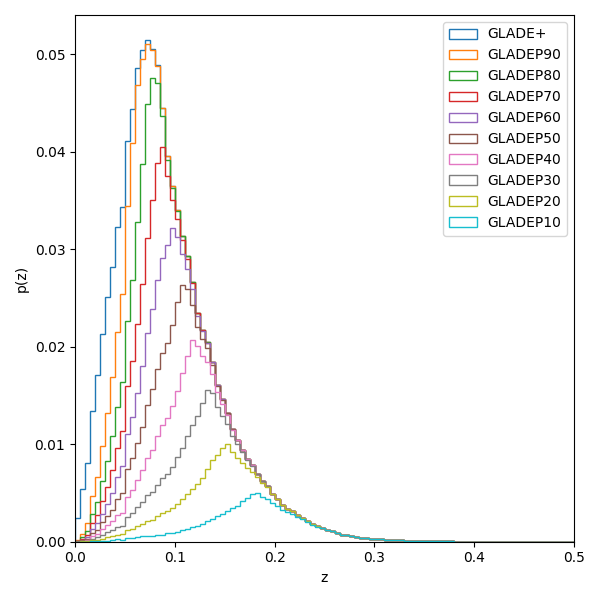
\includegraphics[width=0.7\linewidth]{figures/z_dist_perc.png}
  \caption[Normalized redshift distributions $p(z)$ for the GLADE+ galaxy catalogue and the brightest percentiles.]{Normalized redshift distributions $p(z)$ for the full GLADE+ galaxy catalogue (blue) and the brightest percentiles (other curves). Each subset, labeled “GLADEPXX,” includes only the top XX\% brightest galaxies in the $K$-band. Focusing on increasingly brighter subsets shifts and sharpens the redshift distribution, effectively probing deeper ranges in $z$.}
  \label{fig:z_dist}
\end{figure}

\subsection{Trade-Offs and Limitations}

While bright subsets reduce catalog incompleteness, they may inadvertently exclude genuine host galaxies, especially if those lie in less luminous systems or in underrepresented regions of the catalog. The effectiveness of these cuts depends on the intrinsic distribution of host galaxies, the depth and completeness of the original catalog, and the accuracy of $K$-band photometry. 
%The effectiveness of these cuts therefore depends on:
%\vspace{-1em}
%\begin{itemize}
%  \item The depth and completeness of the original catalog.
%  \vspace{-1em}
%  \item The intrinsic distribution of host galaxies.
%  \vspace{-1em}
%  \item The accuracy of $K$-band photometry.
%\end{itemize}

One major limitation of this approach is that brightest galaxies may not be representative of the overall galaxy population, as they may be biased towards certain types of galaxies or regions of the sky. This effect is however mitigated by the fact that we are using the $K$-band luminosities, which are good tracer for the stellar mass \citep{strazzullo2006near,sureshkumar2021galaxy}, and in turn the overall matter distribution. Furthermore, the bright galaxy subsets are constructed from the \texttt{GLADE+} catalog, which is designed to be a complete and representative sample of galaxies in the local universe. This means that the bright galaxy subsets are likely to be representative of the overall galaxy population, and give a crude estimate of the matter distribution, even if they are not a complete sample.

Estimating the true redshift of a \ac{GW} event by the nearest brightest galaxies is supposed to have a negligible effect on the results. This is because the bright galaxies are more likely to be located in regions of high density, such as galaxy clusters or groups, which are also likely to host \ac{GW} events. This means that the bright galaxies are likely to be located in the same large-scale structure as the \ac{GW} event, and thus provide a good estimate of the redshift of the event. 

One important thing to note is that while the use of a bright subset enhances the completeness of the catalogue at high redshifts, it also introduces a trade-off. If the brightness cut is too restrictive, the exclusion of fainter galaxies may lead to an underrepresentation of the overall matter distribution, potentially biasing the results. One needs to carefully balance these considerations by comparing different brightness thresholds. A moderate brightness cut will maximize the benefit in terms of depth without incurring significant bias.

The appropriate brightness cut can be established only via a set of astrophysics-motivated large-scale simulations. A \ac{GW} \textit{\ac{MDC}} using the simulated \texttt{BUZZARD} galaxy catalog from the \ac{DES} Collaboration~\citep{DES:2019jmj,DES:2021bwg}. It is designed to determine the optimal brightness threshold which maximizes the measurement precision with bright subsets while keeping the biases in control. Tests performed in the process will help refine the methodology and ensure that the improved constraints on the Hubble constant are robust against additional systematic uncertainties.

While the bright galaxy subsets may not be a perfect representation of the overall galaxy population, they are still a useful tool for improving the completeness of the galaxy catalog and reducing the out-of-catalog correction. The error incurred by using the bright galaxies as redhsift tracers maybe small compared to the current errors in luminosity distance measurements from the \ac{GW} events, this may become a problem in the future as the \ac{GW} measurements become more precise. In this case, one may need to use more sophisticated methods to estimate the redshift of the \ac{GW} event, such as more complex models of the galaxy population, but for now this is a good first step towards improving the completeness of the galaxy catalog and reducing the out-of-catalog correction, by leveraging the currently available \ac{EM} data.

%In Chapters~\ref{chap:results} and~\ref{chap:mockdata}, we quantify these trade-offs using both real data and mock catalogs.

\begin{figure}[h!]
  \centering
  \begin{subfigure}{0.32\textwidth}
    \includegraphics[width=\linewidth]{figures/test_frame_g_0.png}
    \label{fig:gladep100}
  \end{subfigure}
  \begin{subfigure}{0.32\textwidth}
    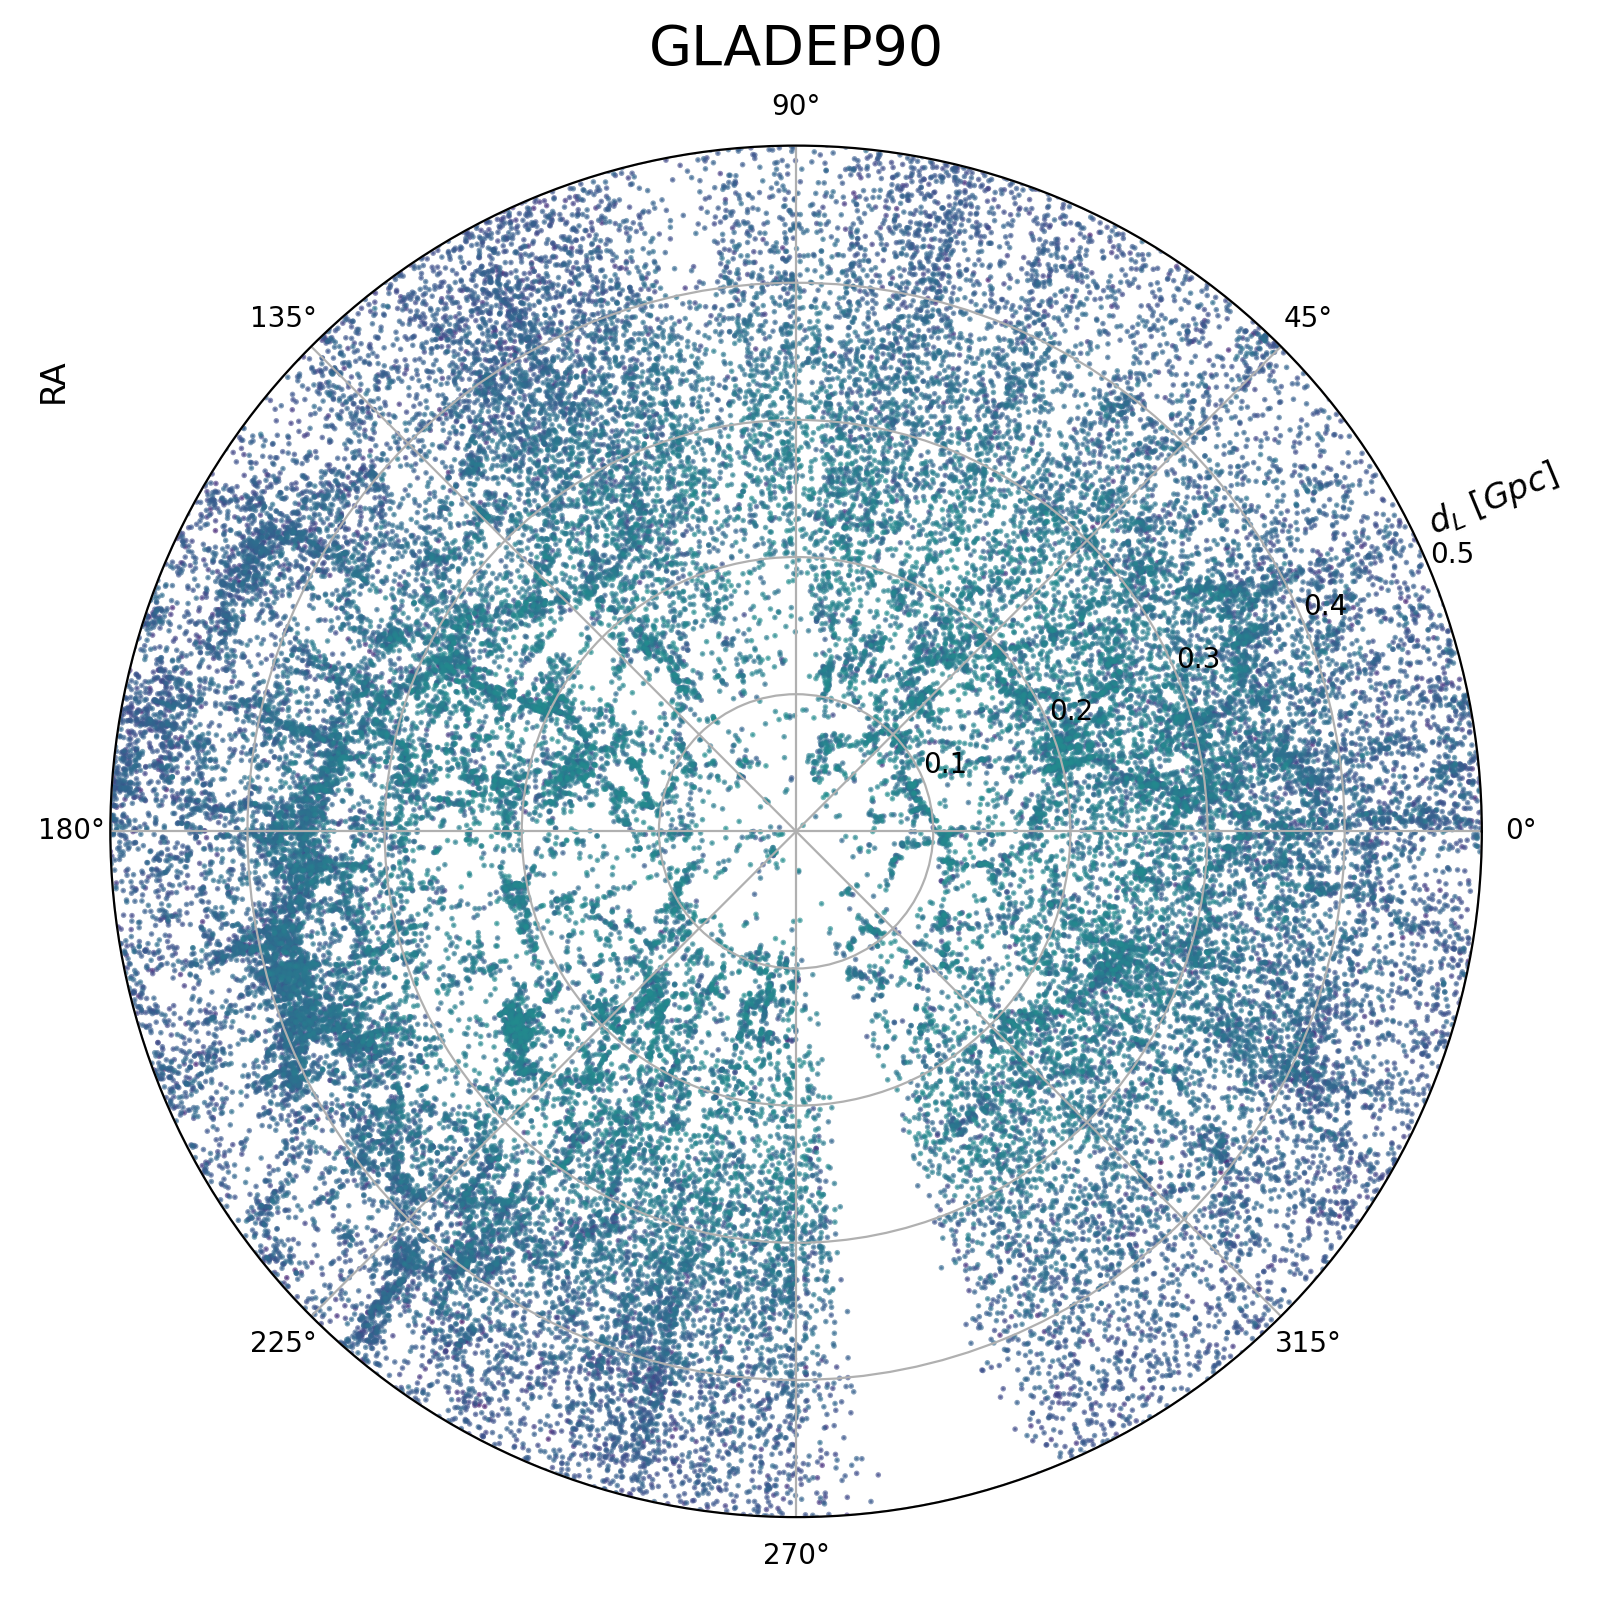
\includegraphics[width=\linewidth]{figures/test_frame_g_1.png}
    \label{fig:gladep90}
  \end{subfigure}
  \begin{subfigure}{0.32\textwidth}
    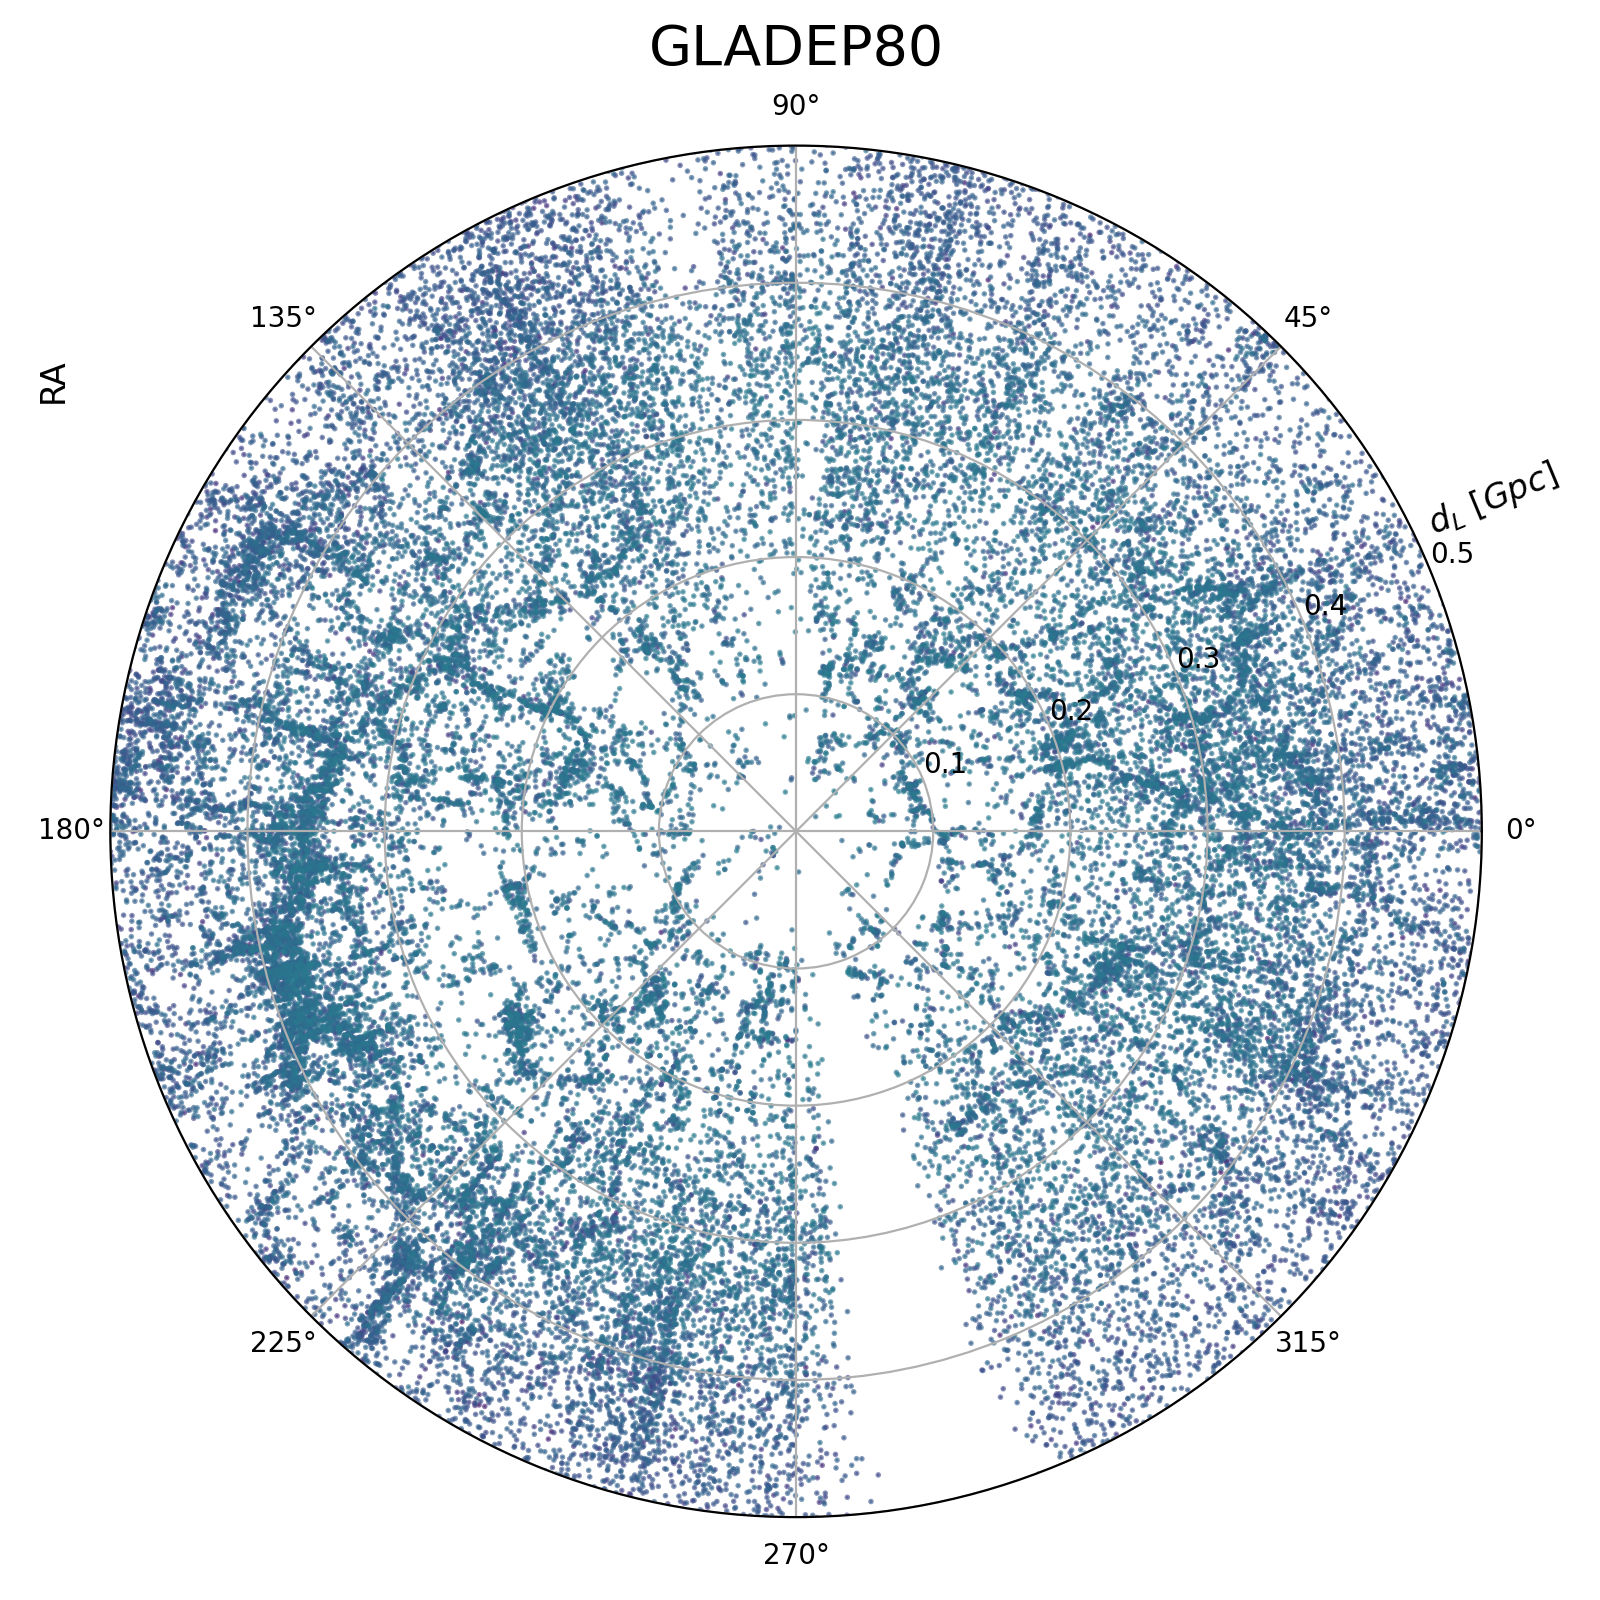
\includegraphics[width=\linewidth]{figures/test_frame_g_2.png}
    \label{fig:gladep80}
  \end{subfigure}
  \vspace{0.5em}
  \begin{subfigure}{0.32\textwidth}
    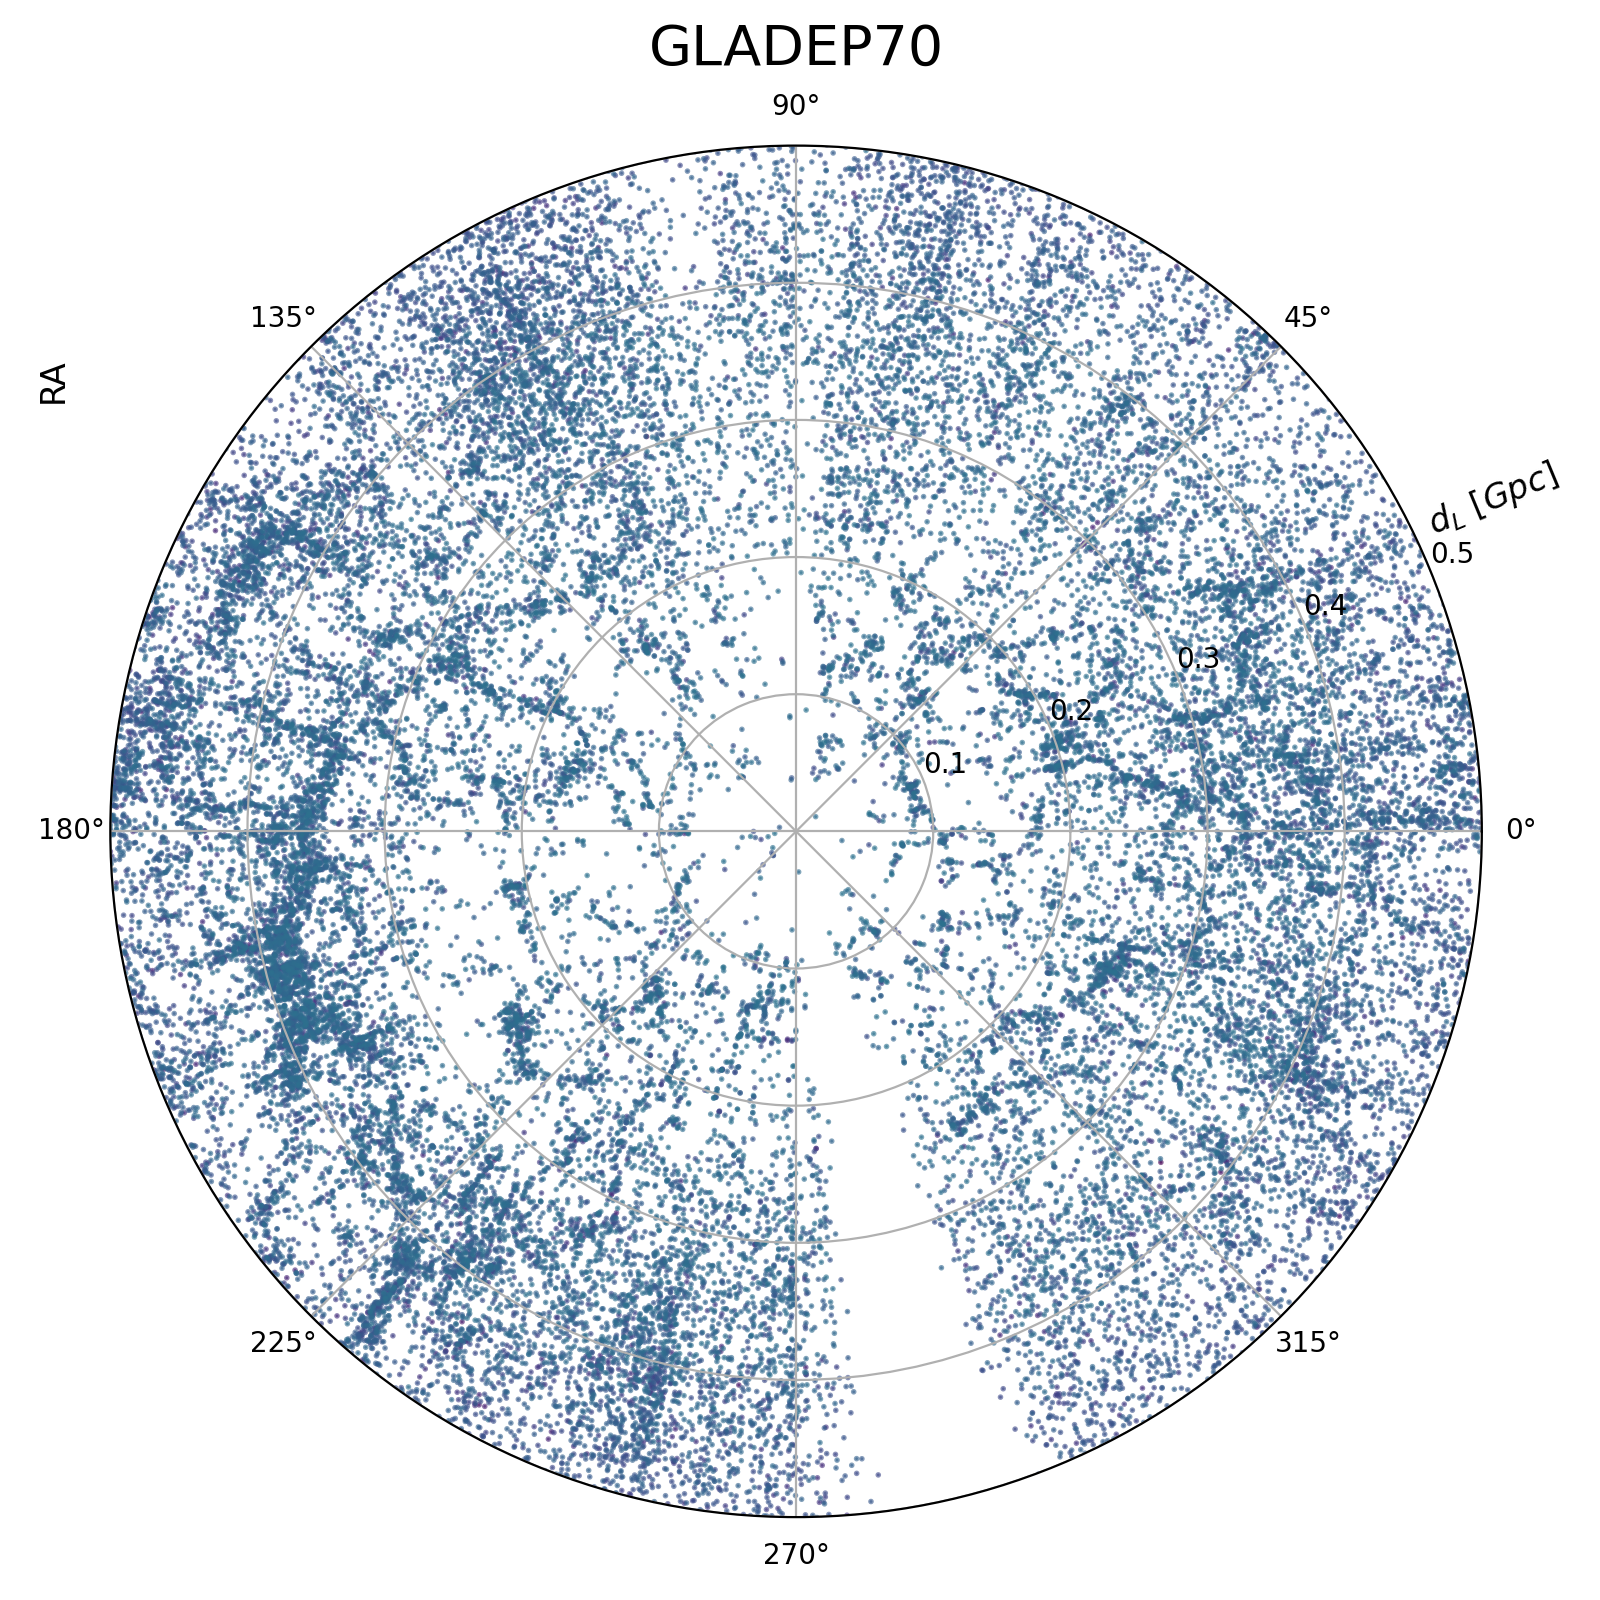
\includegraphics[width=\linewidth]{figures/test_frame_g_3.png}
    \label{fig:gladep70}
  \end{subfigure}
  \begin{subfigure}{0.32\textwidth}
    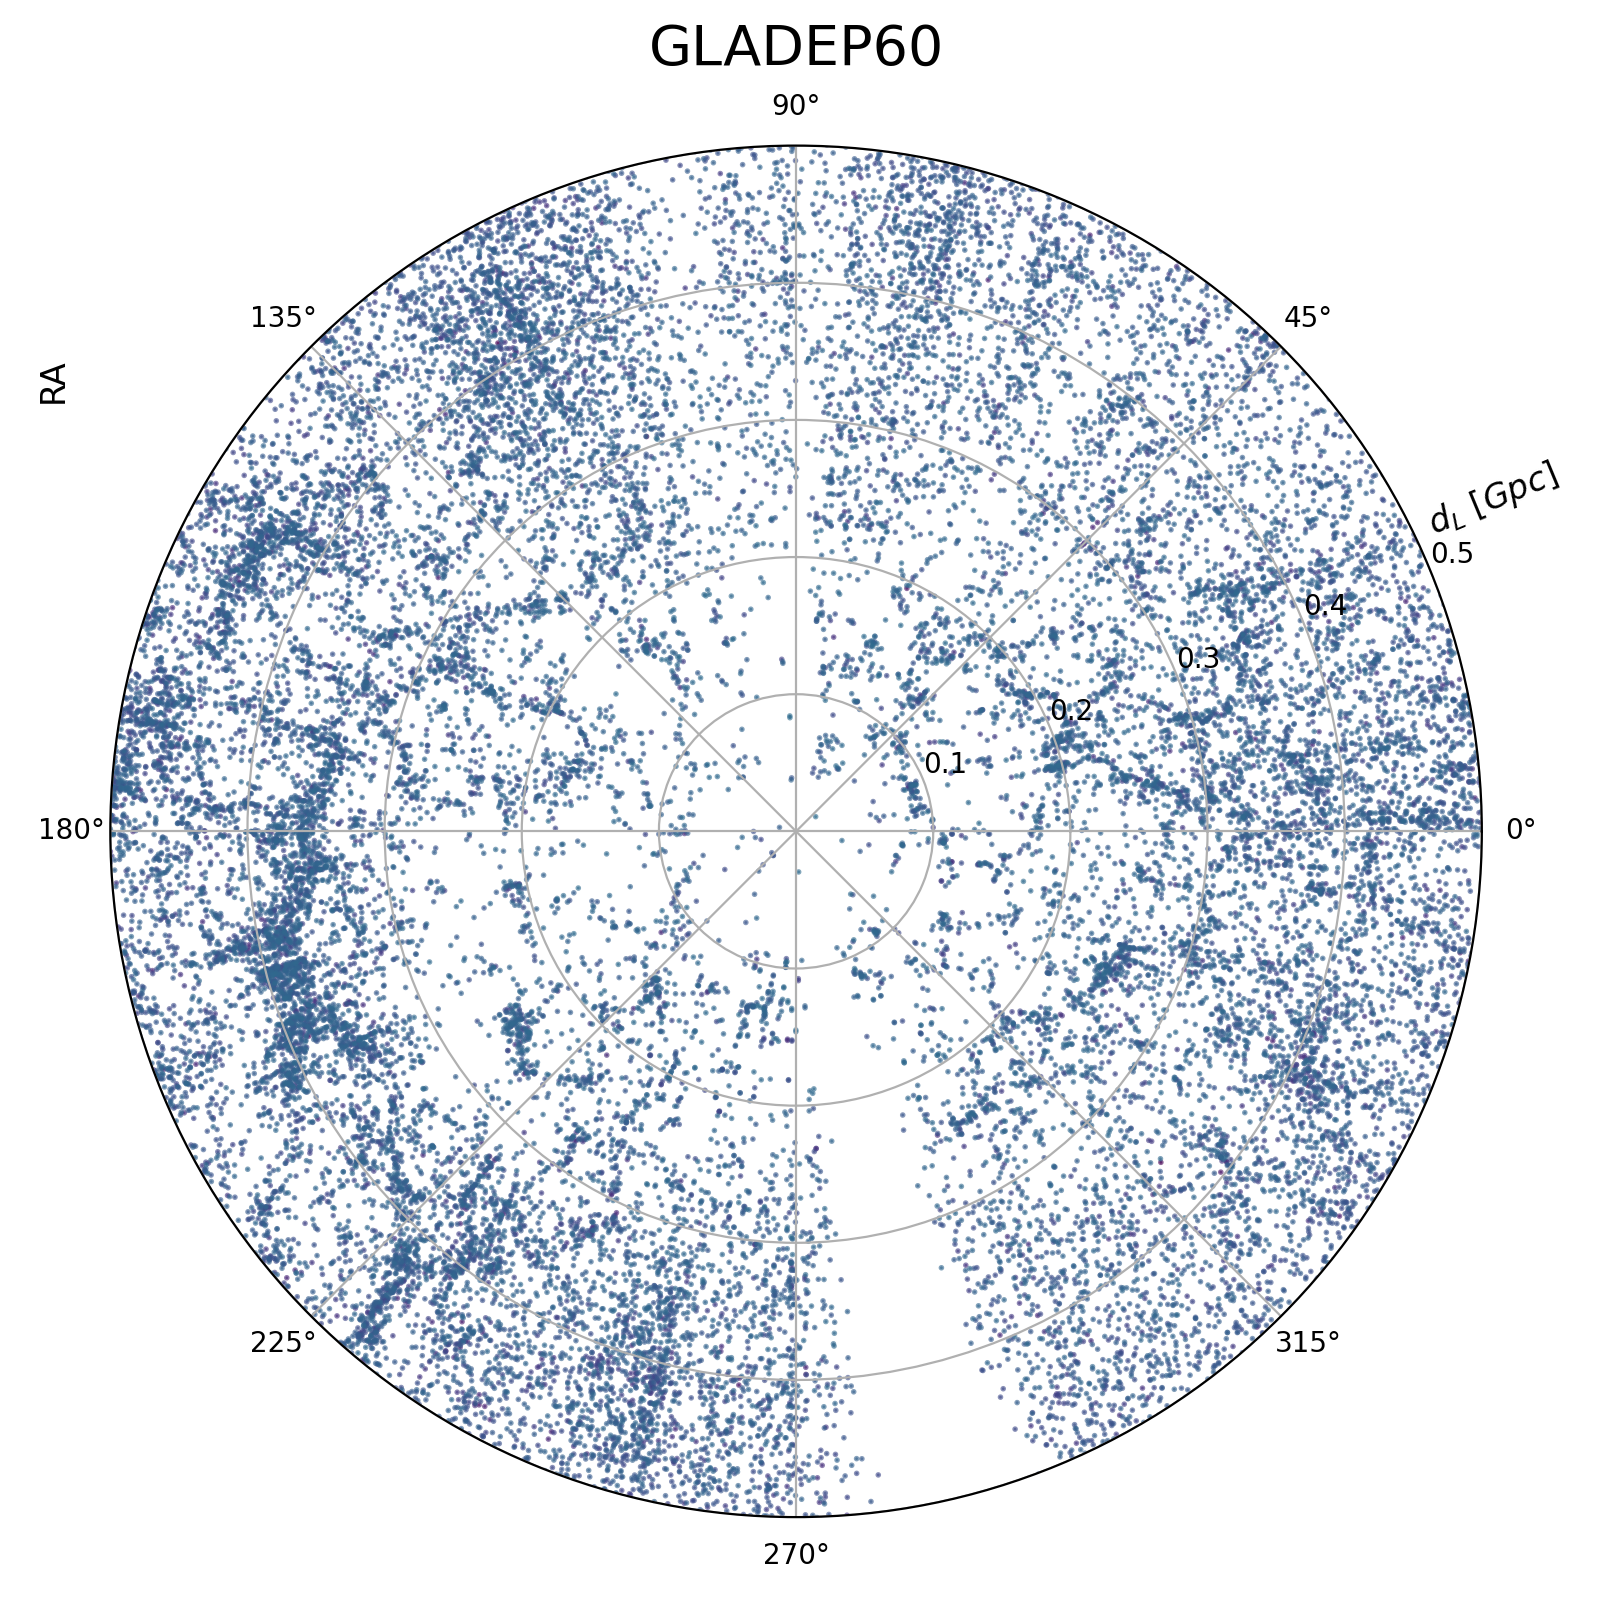
\includegraphics[width=\linewidth]{figures/test_frame_g_4.png}
    \label{fig:gladep60}
  \end{subfigure}
  \begin{subfigure}{0.32\textwidth}
    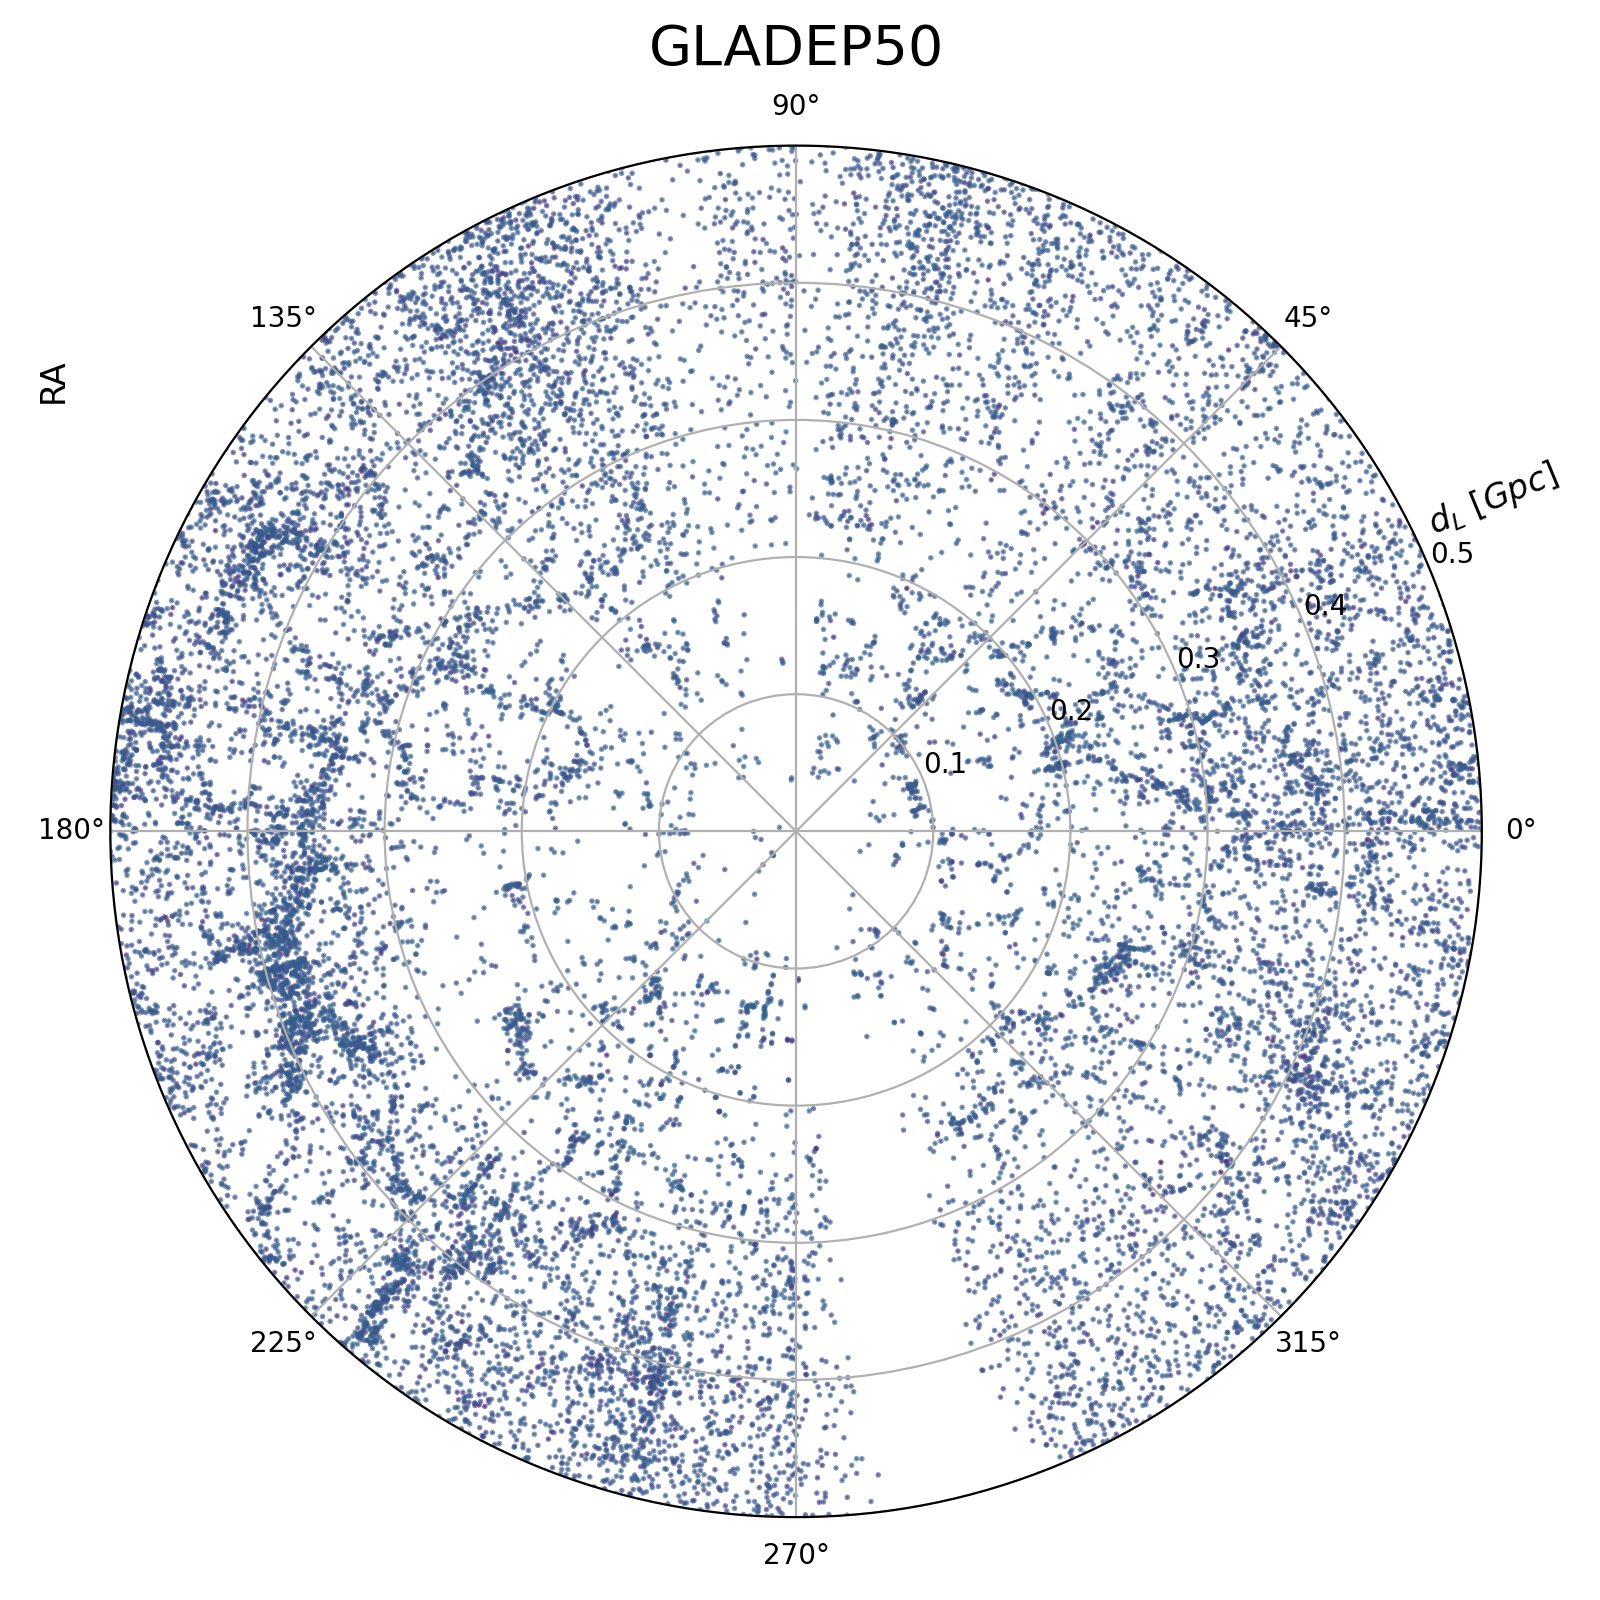
\includegraphics[width=\linewidth]{figures/test_frame_g_5.png}
    \label{fig:gladep50}
  \end{subfigure}
  \vspace{0.5em}
  \begin{subfigure}{0.32\textwidth}
    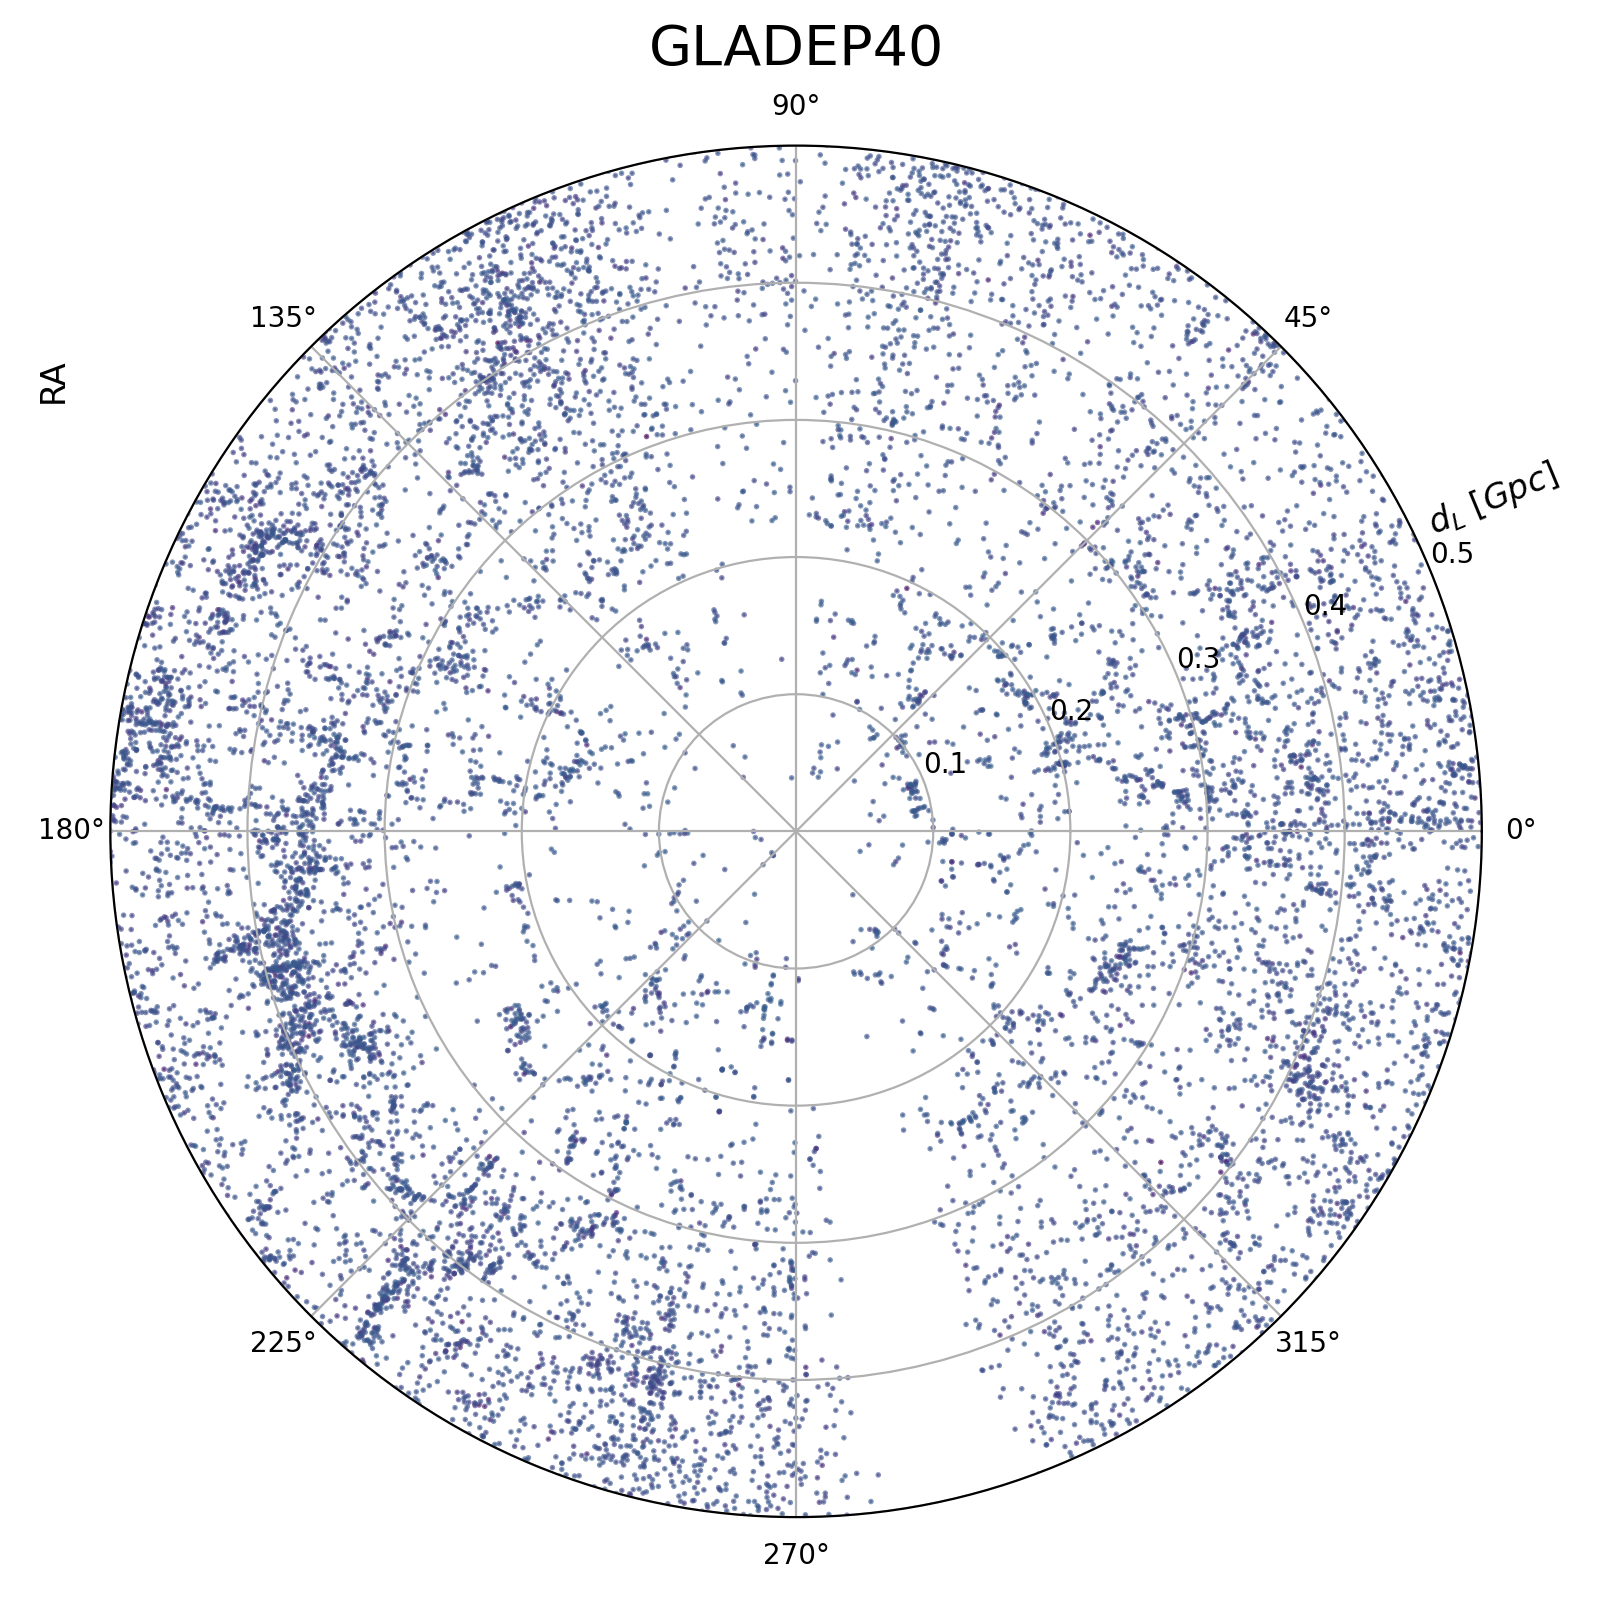
\includegraphics[width=\linewidth]{figures/test_frame_g_6.png}
    \label{fig:gladep40}
  \end{subfigure}
  \begin{subfigure}{0.32\textwidth}
    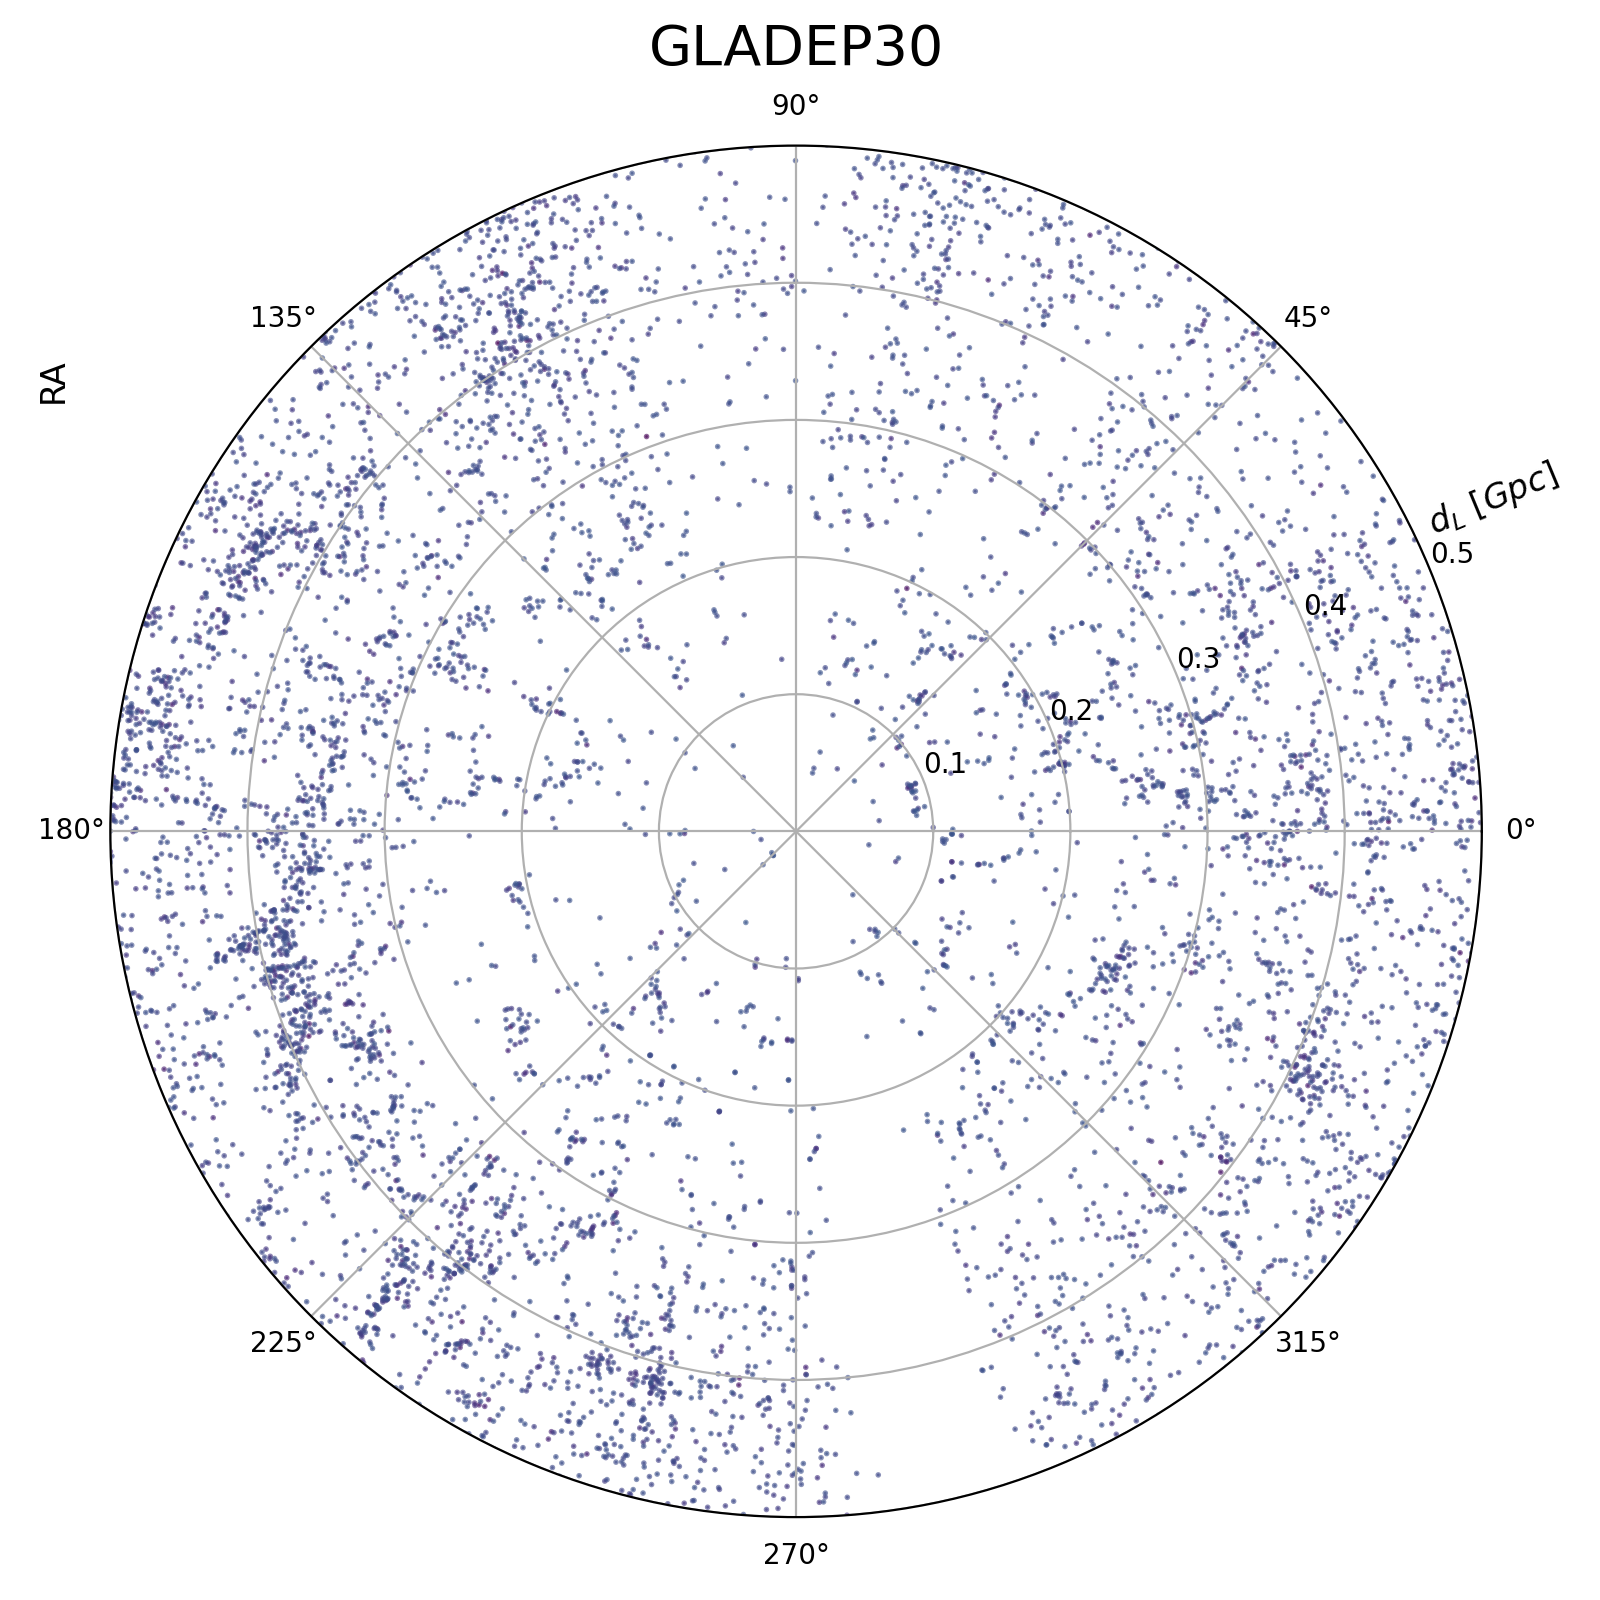
\includegraphics[width=\linewidth]{figures/test_frame_g_7.png}
    \label{fig:gladep30}
  \end{subfigure}
  \begin{subfigure}{0.32\textwidth}
    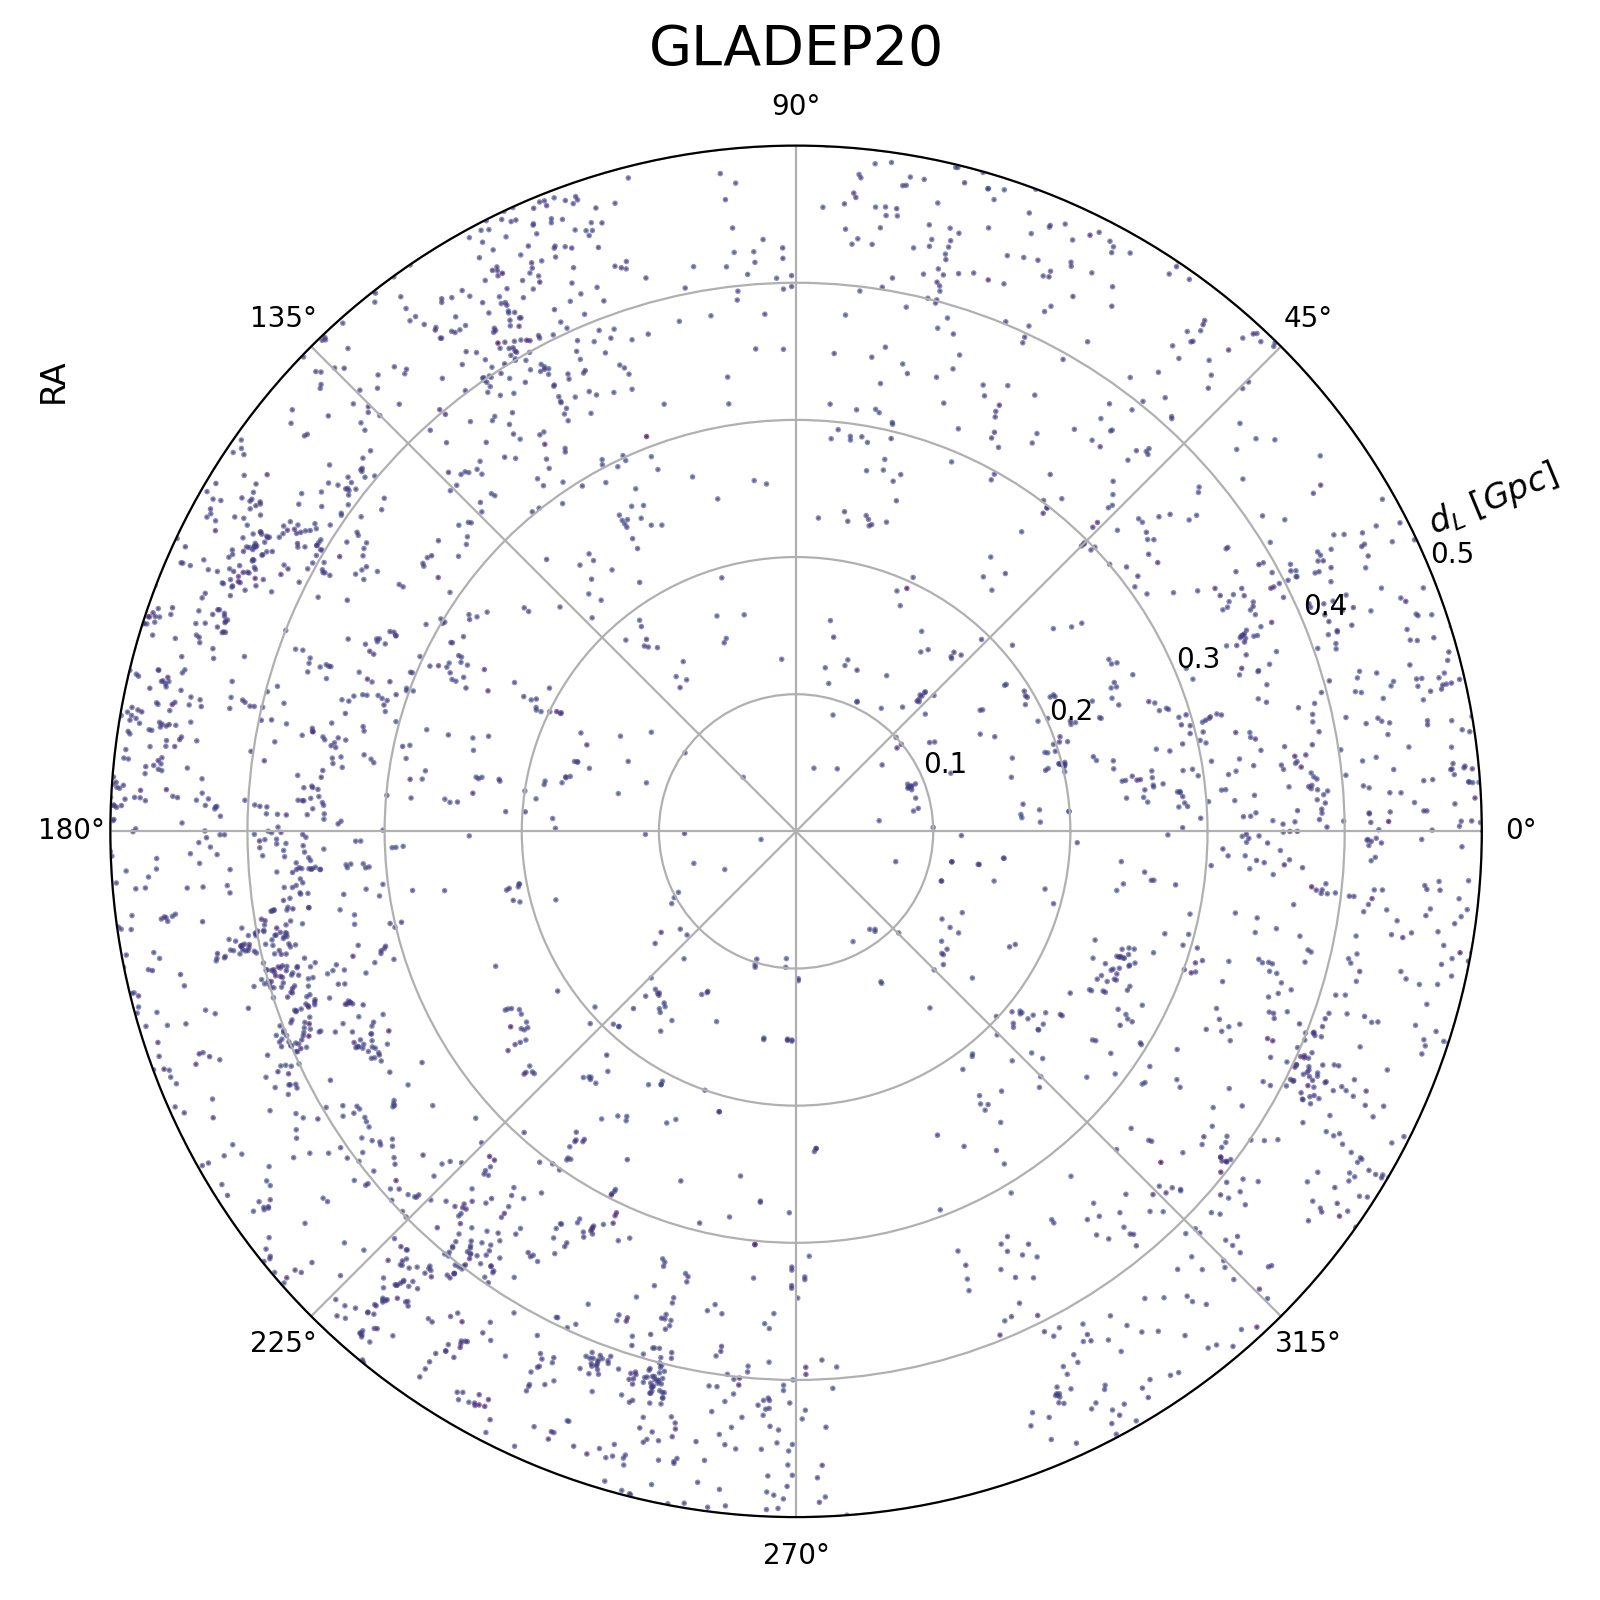
\includegraphics[width=\linewidth]{figures/test_frame_g_8.png}
    \label{fig:gladep20}
  \end{subfigure}

  \vspace{0.5em}

  \begin{subfigure}{0.32\textwidth}
    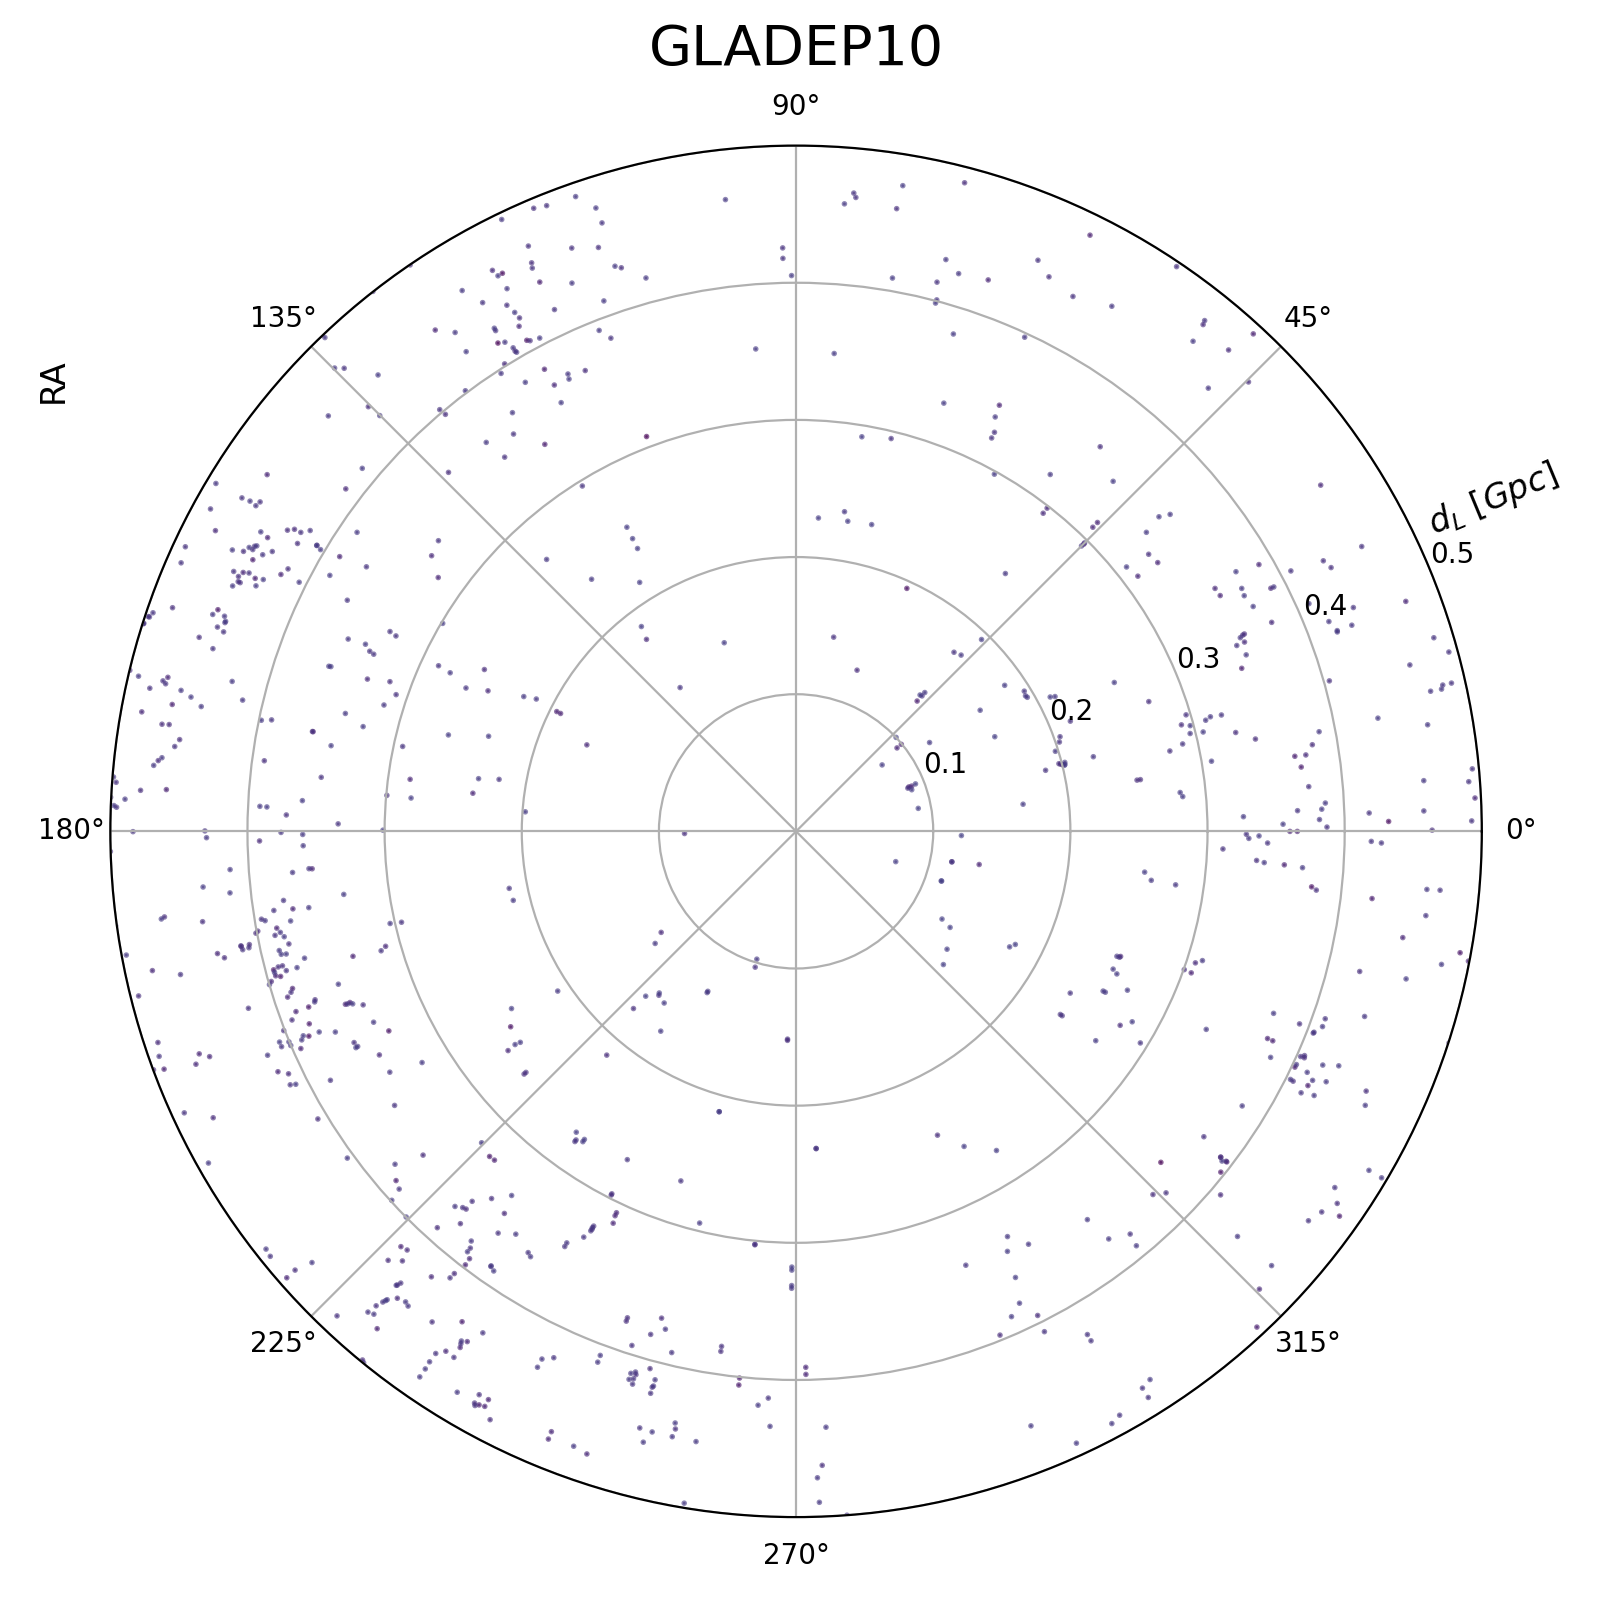
\includegraphics[width=\linewidth]{figures/test_frame_g_9.png}
    \label{fig:gladep10}
  \end{subfigure}
  \begin{subfigure}{0.64\textwidth}
    \centering
    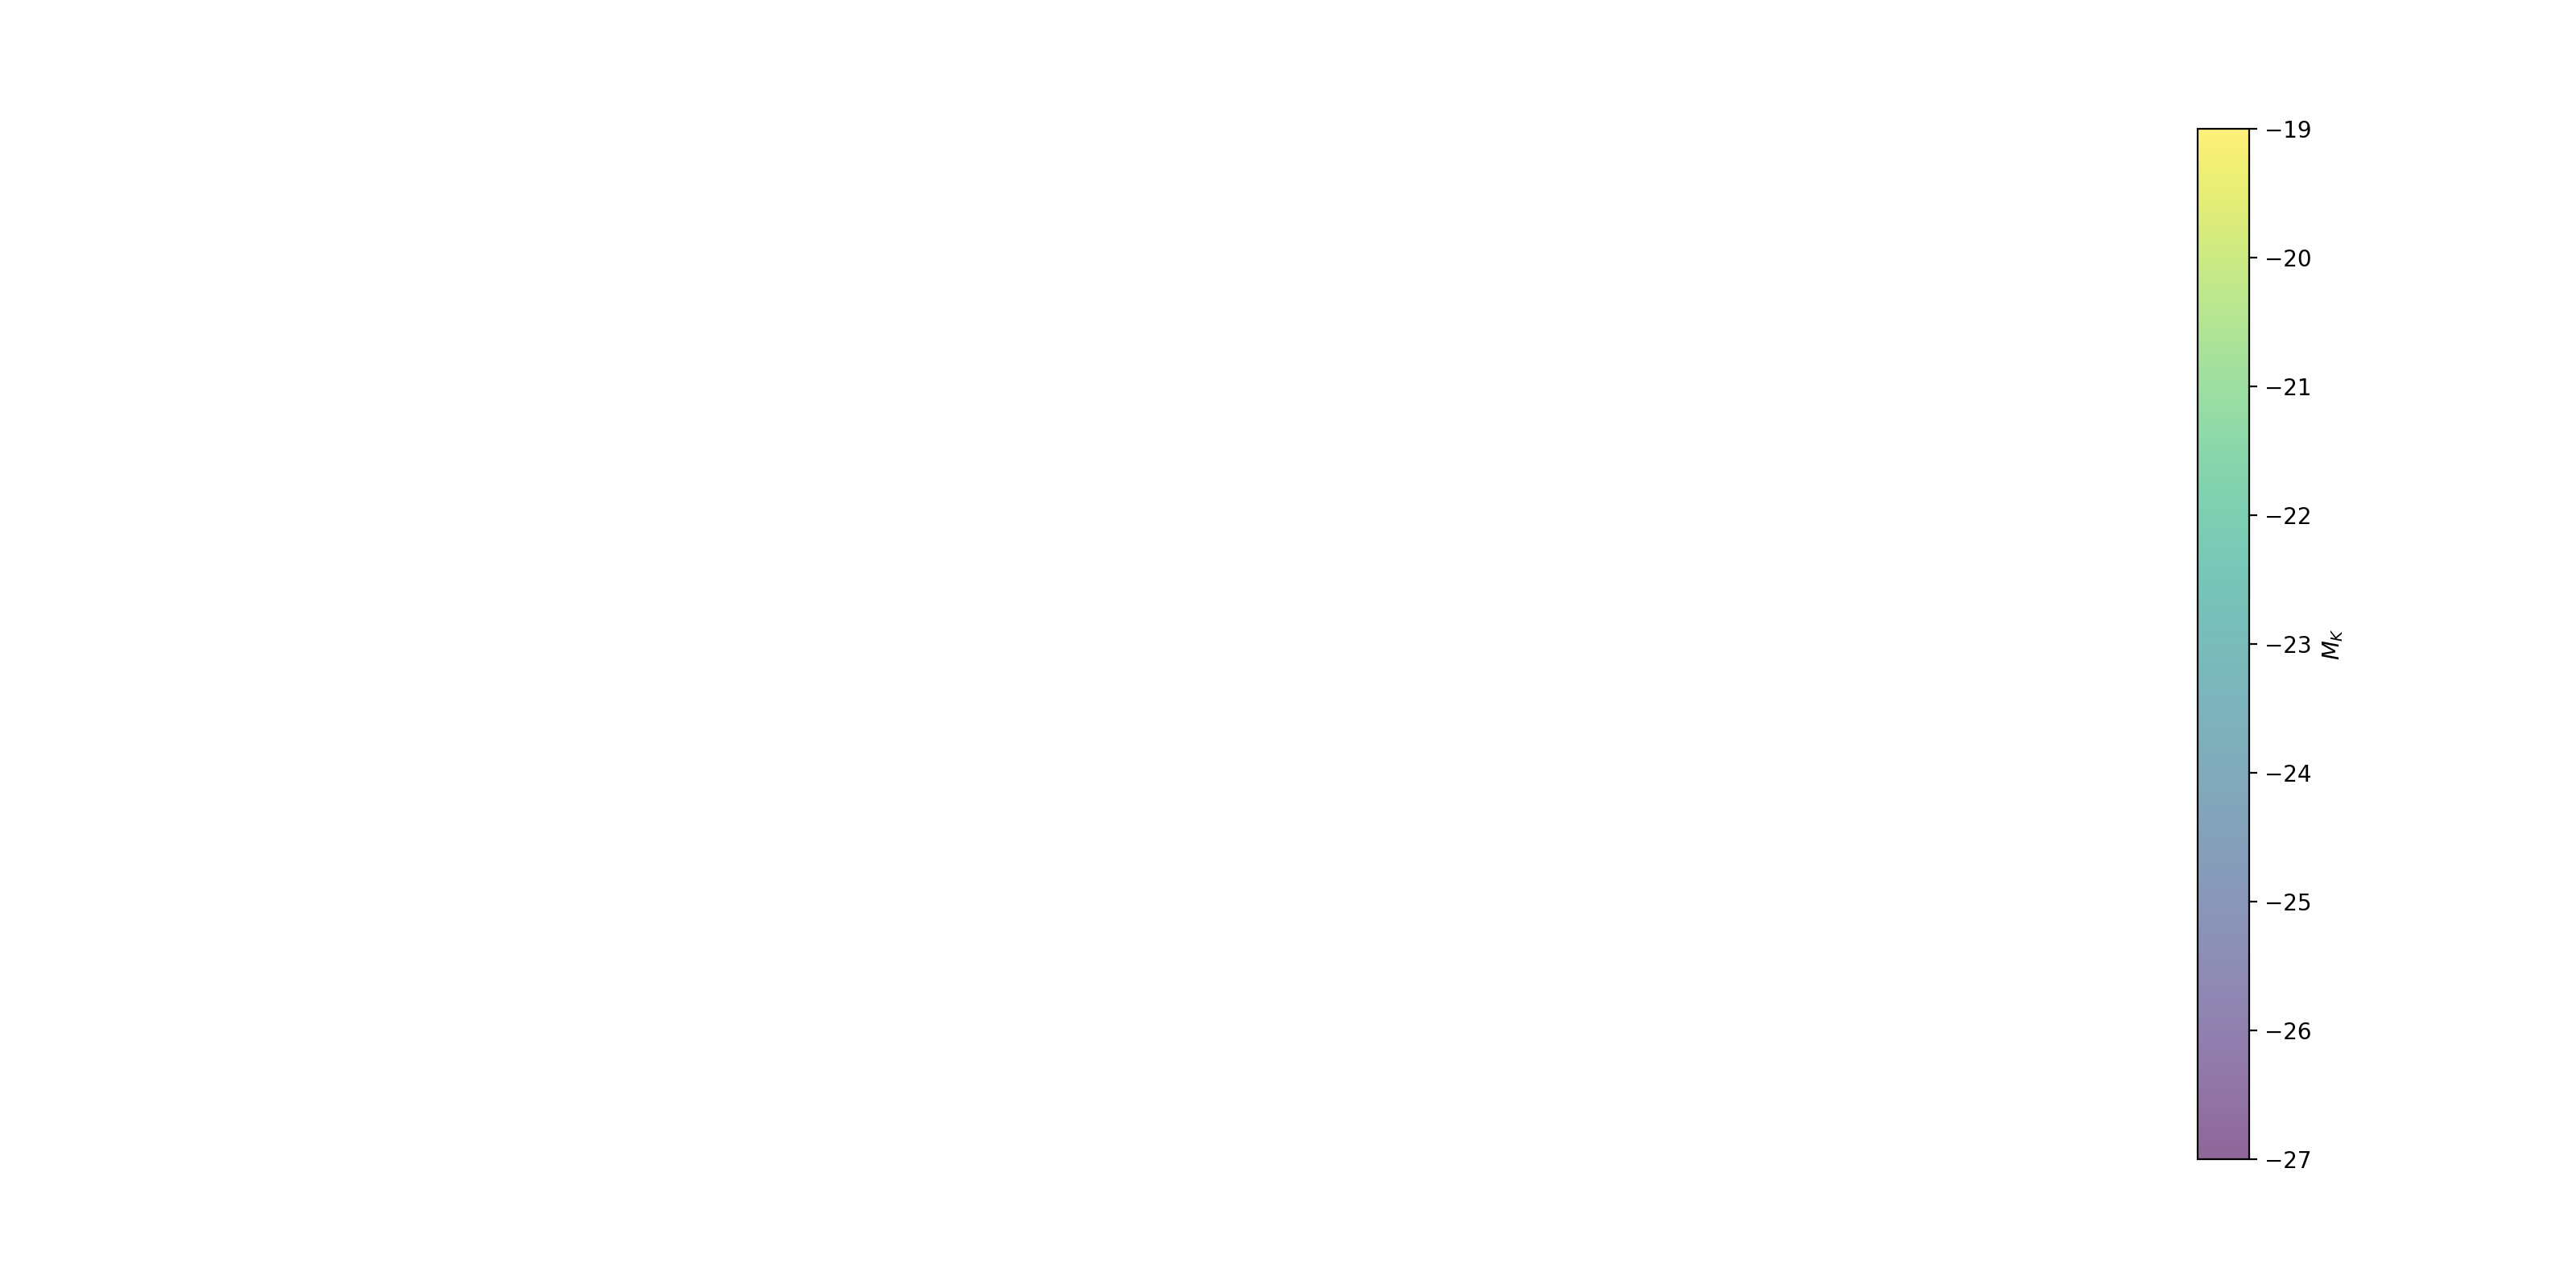
\includegraphics[width=\linewidth]{figures/test_frame_g_colorbar.png}
    \vspace{0.02em}
  \end{subfigure}

  \caption[Spatial distribution of galaxies from the GLADE+ galaxy catalog and its subsets.]{Spatial distribution of galaxies from the GLADE+ catalog and its bright subsets, employed for dark standard siren cosmology. The plots show a 10-degree slice in declination, centered at $0^\circ$, with the radial coordinate representing luminosity distance $d_L$ (in Gpc) and the angular coordinates being right ascension (RA). This shows how the bright galaxies trace the large-scale structure of the universe.}
  \label{fig:dist_gladep}
\end{figure}


\newpage

\section{The \texttt{gwcosmo} Pipeline}
Based on the work presented in \cite{gray2020cosmological,gray2022pixelated,gray2023joint}, \texttt{gwcosmo} is a Python package specifically designed for the joint inference of cosmological parameters using data from standard sirens and galaxy catalogs.  The pipeline employs Bayesian inference techniques to simultaneously constrain cosmological parameters, such as the Hubble constant and dark energy equation of state parameters. It does this using various data inputs, including the gravitational wave strain data from gravitational wave observatories such as LIGO, Virgo, and KAGRA, entries from galaxy catalogs containing photometric or spectroscopic redshift information, as well as other relevant galaxy properties, and \ac{CBC} source population models. 

\texttt{gwcosmo} represents a significant advancement in extracting cosmological information especially from \ac{CBC} events that lack unique \ac{EM} counterparts. It addresses the challenge of redshift inference in dark siren cosmology by statistically marginalizing over potential host galaxies from a flux-limited catalog. This is achieved through hierarchical Bayesian modeling that incorporates \ac{GW} strain data, the spatial and redshift distribution of galaxies, and astrophysical population models.

The pipeline is designed to be flexible and extensible, allowing users to customize the models and priors used in the analysis. It also provides tools for visualizing the results, including posterior distributions and confidence intervals for the inferred parameters. The package is built on top of established libraries such as \texttt{numpy}, \texttt{scipy}, and \texttt{matplotlib}, making it accessible to researchers familiar with these tools.
The \texttt{gwcosmo} pipeline is a particularly useful tool in the intersection of gravitational wave astronomy and cosmology, as it enables the extraction of valuable cosmological information from gravitational wave events, which can complement traditional methods of measuring cosmological parameters. The package is actively maintained and updated to incorporate new developments in both gravitational wave detection and cosmological modeling, ensuring that it remains a relevant tool for researchers in the field.

\subsection{Bayesian Framework: \textbf{TO BE UPDATED} (see gwcosmo paper)}
The goal is to evaluate the posterior distribution:
\begin{equation}
p(\Lambda \mid \{d_{\text{GW}}\}, \{d_{\text{EM}}\}) \propto p(\Lambda) \, p(\{d_{\text{GW}}\}, \{d_{\text{EM}}\} \mid \Lambda),
\end{equation}
where:
\begin{itemize}
  \vspace{-1em}
  \item $\Lambda$ are the hyperparameters of interest (e.g., cosmological parameters, population hyperparameters),
  \vspace{-1em}
  \item $d_{\text{GW}}$ are the GW observables (e.g., luminosity distance posteriors),
  \vspace{-1em}
  \item $d_{\text{EM}}$ are the galaxy catalogue data (e.g., redshifts, magnitudes, positions).
\end{itemize}

The likelihood is approximated by marginalizing over all galaxies $k$ within the GW localization volume:
\begin{equation}
p(\Lambda \mid \{d_{\text{GW}}\}, \{d_{\text{EM}}\}) \propto \prod_{i} \sum_{k} w_k \, p(d_{\text{GW},i} \mid z_k, \Lambda),
\end{equation}
where $w_k$ is the weight assigned to each galaxy, typically modeled based on a proxy for host probability (e.g., luminosity in a selected band, merger rate evolution).

\subsection{Key Features of \texttt{gwcosmo}}
Some of the key features of the \texttt{gwcosmo} pipeline include:
\begin{itemize}
  \item \textbf{Joint Population + Cosmology Inference:} Simultaneously samples over cosmological parameters and population hyperparameters, avoiding bias from fixed population assumptions.
  \item \textbf{Galaxy Catalogue Weighting:} Utilizes \ac{LOS} redshift priors constructed from galaxy distributions, incorporating completeness corrections based on flux thresholds.
  \item \textbf{Selection Effects:} Corrects for GW detector sensitivity and incompleteness in galaxy catalogues by modeling detection probabilities and magnitude limits.
\end{itemize}

\subsection{Implementation and Applications}

The pipeline is implemented in Python and uses \ac{KDE} of \ac{GW} posteriors and efficient catalog summation to handle discrete and incomplete galaxy data. The most recent version was applied by \cite{gray2023joint} to reanalyze 47 events from the \ac{GWTC}-3 catalog using the \texttt{GLADE+} galaxy catalog, yielding an updated measurement of the Hubble constant:
$$
H_0 = 69^{+12}_{-7}~\text{km s}^{-1}~\text{Mpc}^{-1}.
$$

\texttt{gwcosmo} is publicly available and is expected to be a useful tool for future gravitational-wave cosmology with upcoming detector runs and deeper galaxy surveys.

\section{\ac{LOS} Redshift Prior}
We base our analysis on the \texttt{gwcosmo} pipeline \citep{gray2020cosmological,gray2022pixelated,gray2023joint}, which relies on a precomputed \ac{LOS} redshift prior, a prior on the \ac{GW} signal's redshift and direction. This \ac{LOS} redshift prior is used in tandem with the luminosity distance posterior from the \ac{GW} signal, to get a measurement for the Hubble constant $H_0$.

\subsection{\ac{LOS} Redshift Prior Construction}
The \ac{LOS} redshift prior is constructed from the \texttt{GLADE+} galaxy catalog, which contains a wealth of information about the galaxies in the local universe. The redshift prior is constructed by taking into account the distribution of galaxies along the line of sight to the \ac{GW} event, as well as their luminosity and redshift. This allows us to obtain a more accurate estimate for the redshift of the \ac{GW} signal, which is crucial for cosmological measurements. The prior is constructed by dividing the sky into HEALPix pixels, and computing the redshift distribution of galaxies in each pixel. The redshift prior is then weighted using the luminosity of the potential host galaxies, allowing us to obtain a more accurate estimate for the Hubble constant.

Furthermore, the prior accounts for the incompleteness of the galaxy catalog, using source population models and the magnitude threshold calculated per pixel, which is particularly important for high-redshift events where the number of galaxies is significantly reduced. This allows us to separate the \ac{LOS} redshift prior into an in-catalog and out-of-catalog contribution.

Taking into account, the fact that the host galaxy can be present, marked as $G$, or not, marked as $\bar{G}$, inside the catalog, one can write the \ac{LOS} redshift prior as:
\begin{align}
  p(z|\Omega_i, \Lambda, s, I) =& \iint \sum_{g=G,\bar{G}} p(z, M, m,g|\Omega_i, \Lambda, s, I)~dM dm \\
  =&~p(G|\Omega_i, \Lambda, s, I) \iint p(z, M, m|G,\Omega_i, \Lambda, s, I)~dM dm \nonumber \\
  &+ p(\bar{G}|\Omega_i, \Lambda, s, I) \iint p(z, M, m|\bar{G},\Omega_i, \Lambda, s, I)~dM dm
\end{align}

The first term in the equation represents the contribution from galaxies that are present in the catalog, while the second term represents the contribution from galaxies not present in the catalog. The two terms are weighted by their respective probabilities of being present or not in the catalog. The terms inside the integral are the priors on the redshift $z$, absolute magnitude $M$, and apparent magnitude of the galaxies $m$, informed by the galaxy catalog, within the sky area covered by pixel $i$. Here the parameters $G/\bar{G}$ give the presence or absence of the galaxy in the catalog, $\Omega_i$ the sky location of the \ac{GW} event, $\Lambda$ the cosmological and population hyperparameters of interest, $s$ the presence of a \ac{GW} source, and $I$ the additional assumptions which are not excplicitly expressed. One also needs to marginalize over the absolute magnitude $M$ and the apparent magnitude $m$ of the galaxy, as these determine, to the leading order, which galaxiess are present in a flux-limited \ac{EM} survey \citep{gray2023joint}.

%\subsubsection{In-Catalog Contribution}
The integral in the in-catalog term can be expressed as the sum over the possible host galaxies in the catalog, weighted by their respective probabilities of being the host galaxy. These galaxies are weighted by their luminosity, which is a function of the absolute magnitude and redshift. The rationale being that the more luminous, and thus heavier galaxies are more likely to host \ac{CBC} events, and therefore contribute more to the \ac{LOS} redshift prior. This reduces the in-catalog part to a wieghted sum over the galaxies in the catalog, where the galaxies are treated as point sources modeled by a Gaussian. This term can thus be expressed as:
\begin{align}
  \iint p(z, M, m|G,\Omega_i, \Lambda, s, I)~dM dm =& \frac{1}{p(s|G,\Omega_i, \Lambda, I)N_{gal}(\Omega_i)} \nonumber\\ 
  &\times \sum_{k}^{N_{gal}(\Omega_i)} p(z|\hat{z}_k) p(s|z, M(z, \hat{m}_k, \Lambda), \Lambda, I)
\end{align}
where the term $p(z|\hat{z}_k)$ represents the probability of a galaxy being at redshift $z$, given its observed redshift $\hat{z}_k$. This term is used to weight the contribution from each galaxy in the catalog, based on its observed redshift.

%\subsubsection{Out-of-Catalog Contribution}
The integral in the out-of-catalog term marginalizes over the possible host galaxies not present in the catalog. This term is more complex, as it requires a model for the distribution of galaxies in the universe, which is not directly available from the catalog. We use a Schechter luminosity function to model the distribution of galaxies in the universe, which allows us to estimate the contribution from galaxies outside the catalog. The out-of-catalog term can be expressed as:
\begin{align}
  \iint & p(z, M, m|\bar{G},\Omega_i, \Lambda, s, I)~dM dm \nonumber \\
  &= \frac{1}{p(s|\bar{G},\Omega_i, \Lambda, I)p(\bar{G}|\Omega_i, \Lambda, I)} \nonumber \\ 
  &~~~\times \Bigg[\Theta[z_{cut} -z] \int_{M(z,m_{th}(\Omega_i), \Lambda)}^{M_{max}(H_0)} p(z,M|\Lambda, I) p(s|z,M,\Lambda,I)~dM \nonumber \\
  &\qquad \quad + \Theta[z-z_{cut}] \int_{M_{min}(H_0)}^{M_{max}(H_0)} p(z,M|\Lambda, I) p(s|z,M,\Lambda,I)~dM \Bigg]
\end{align}
Here we also account for the \ac{EM} selection effects of the catalog. Due to the flux limited nature of the galaxy catalog, the probability of a galaxy being present in the catalog depends on the galaxy's apparanet magnitude, and whether it is greater or smaller than apparent magnitude threshold of the catalog along the same line of sight, $m_{th}(\Omega_i)$. The Heaviside function $\Theta$ is used to separate the two cases of the out-of-catalog contribution, depending on whether the redshift $z$ is below or above a certain threshold $z_{cut}$. This is due to to the exclusion of galaxies with redshift $z$ greater than $z_{cut}$ from the catalog, which is a result of unreliable redshift or color information at these higher redhsifts. 

The term $p(s|z,M,\Lambda,I)$ is the weighting factor for the contribution from each galaxy, based on its luminosity and redshift. The galaxies are weighted by their luminosity in the $K$-band, which is a good tracer of the mass of the galaxies \citep{strazzullo2006near,sureshkumar2021galaxy}. Furthermore, the merger host probability is also taken into account, which is a function of the redshift. This is modeled by a Madau-Dickinson merger rate evolution model \citep{madau2014cosmic}, which describes the evolution of the merger rate with redshift, discussed in Section \ref{sec:source_population}. The term $p(s|z,M,\Lambda,I)$, also incorporates the source population models, used to pouplate the out-of-catalog contribution. These models are also discussed in Section \ref{sec:source_population}.

The term $p(z,M|\Lambda, I)$ represents the luminosity funtion of the galaxies, taken to be the Schechter luminosity function, discussed in Section \ref{sec:luminosity_function}. The integration limits are set by the minimum and maximum absolute magnitudes of the galaxies, $M_{min}(H_0)$ and $M_{max}(H_0)$. These are $H_0$-dependent, as the parameters of the Schechter luminosity function are also $H_0$-dependent, but the final distribution remains insensitive to the exact values of $H_0$ \citep{gray2023joint}.

\section{Results}
In this chapter we present the main outcomes of our analysis: how applying brightness cuts to the \texttt{GLADE+} catalog alters \ac{LOS} redshift prior for individual events, how these modified priors propagate into the inferred posterior on the Hubble constant $H_0$, and where the optimal balance lies between catalog depth and sampling variance.

To test the impact of catalog completeness, we apply successive cuts to the galaxy catalog by selecting only the brightest $XX\%$ of galaxies in $K$-band luminosity, forming subsets labeled \texttt{GLADEPXX}. This process shifts the effective magnitude threshold upward, reducing the number of galaxies but improving the catalog's completeness above the cut.

\subsection{\ac{LOS} Redshift Prior}
Figure~\ref{fig:los_prior_gw170809} shows the LOS redshift prior for the event GW170809 under different catalog cuts. Bright galaxy subsets (e.g., \texttt{GLADEP20}) result in sharper redshift distributions and reduce the weight of the out-of-catalog term. The low-$z$ tail contributed by faint galaxies in the nearby universe is also suppressed. Notably, these priors maintain consistency in shape, indicating that bright galaxies are reliable tracers of large-scale structure. The application of a brightness cut significantly modifies the \ac{LOS} redshift distribution. Specifically, the bright galaxy subsets yield an amplified redshift prior at higher distances, effectively extending the reach of the catalogue, somewhat mitigating the incompleteness issues that arise at deeper redshifts. This behavior is qualitatively consistent across events.

\begin{figure}[ht]
  \centering
  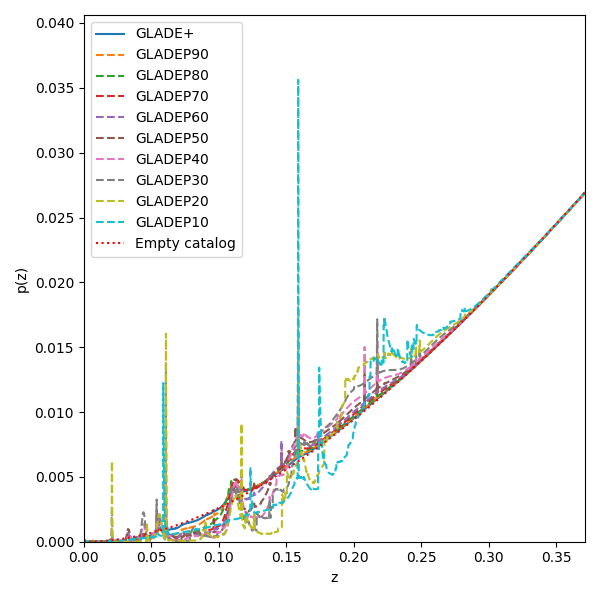
\includegraphics[width=0.7\textwidth]{figures/GW170809_zprior.png}
  \caption[LOS redshift prior for GW170809 for different brightness-ranked \texttt{GLADE} subsets]{LOS redshift prior for GW170809 for different brightness-ranked \texttt{GLADE} subsets. The full \texttt{GLADE+} catalog (solid blue) is compared to the different subsets. Applying a brightness cut amplifies the prior at higher distances, extending the effective reach of the catalog and partially mitigating incompleteness at greater redshifts.}
  \label{fig:los_prior_gw170809}
\end{figure}

\subsection{Hubble Constant Posterior}
Once one has the \ac{LOS} redshift prior, one can use it to compute the posterior distribution of the Hubble constant $H_0$ given the \ac{GW} event data, as the relation between the redhsift $z$, luminosity distance $d_L$ and the Hubble constant $H_0$ is given by:
\begin{align}
  d_L = \frac{c(1+z)}{H_0} \int_0^z \frac{dz'}{\sqrt{(1+z')^3\Omega_m + \Omega_\Lambda}}
\end{align}
for a flat $\Lambda$CDM cosmology. At lower redshifts, this can be simplified to:
\begin{align}
  d_L \approx \frac{cz}{H_0}
\end{align}
Thus the \ac{LOS} redshift prior, $p(z|\Omega_i, \Lambda, s, I)$, and the luminosity distance posterior, $p(d_L,\Omega\mid\mathrm{GW})$, from the \ac{GW} event data can be combined to obtain the posterior distribution of $H_0$, which can then be used to obtain constraints on the value of $H_0$.

\begin{figure}[h!]
  \centering
  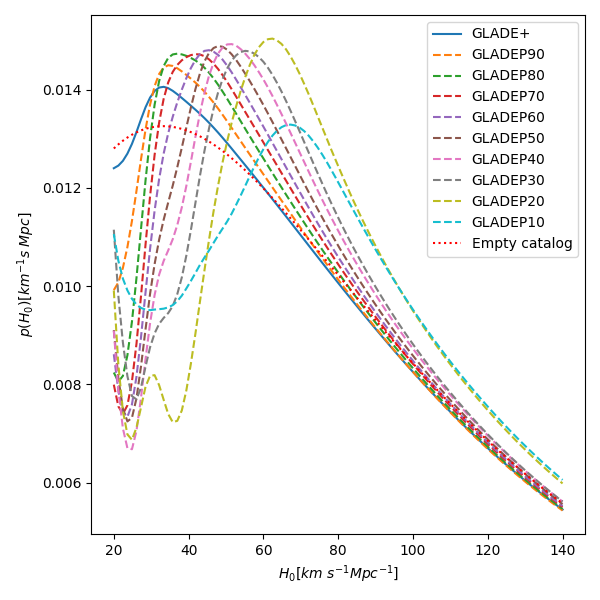
\includegraphics[width=0.7\textwidth]{figures/GW170809_H0.png}
  \caption[$H_0$ posterior distributions for GW170809 using full and brightness-cut galaxy catalogs.]{$H_0$ posterior distributions for GW170809 using full and brightness-cut galaxy catalogs. \texttt{GLADEP20} yields the tightest credible interval. \texttt{GLADEP10} suffers from sparse sampling.}
  \label{fig:h0_gw170809}
\end{figure}

Figure~\ref{fig:h0_gw170809} shows the resulting $H_0$ posteriors for GW170809 under various catalog cuts. As the catalog is restricted to brighter galaxies, the $H_0$ posterior becomes increasingly narrow. For example, \texttt{GLADEP20} yields a visibly tighter posterior compared to the full \texttt{GLADE+}, with minimal shift in the median. However, the most aggressive cut (\texttt{GLADEP10}) introduces broader tails, likely due to insufficient galaxy sampling in the localization volume. (\textbf{LINK TO THE 20\% LIMIT IN BUZZARD?})

We repeat this procedure for a subset of \ac{BBH} events from \ac{GWTC} that meet our selection criteria. Figure~\ref{fig:h0_cumulative} shows the combined $H_0$ posterior from the selected dark siren events using the full \texttt{GLADE+} catalog and the different subsets.

Table~\ref{tab:h0_stats} summarizes the $H_0$ posteriors for all cuts. The uncertainty is minimized around the \texttt{GLADEP20} subset, showing 30-40\% tighter contraints, while median values shift towards a higher value. For less extreme cuts, the median values doesn't show a huge shift. This suggests that moderate brightness cuts improve precision without introducing systematic bias.

\begin{figure}[ht]
    \centering
    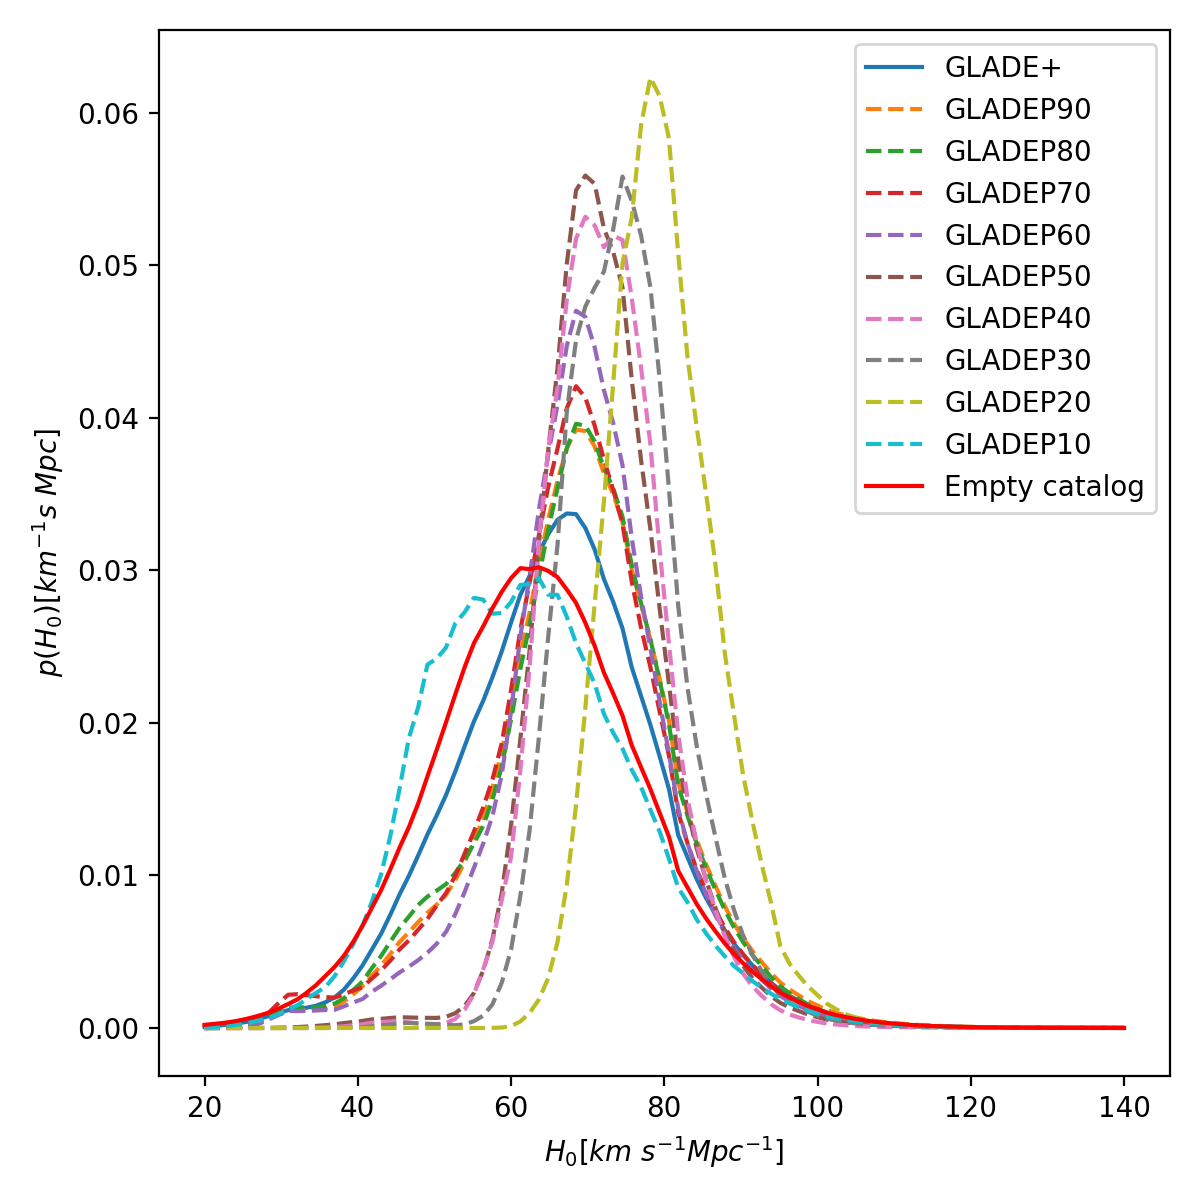
\includegraphics[width=0.7\textwidth]{figures/percentile_full_dict.png}
    \caption[Cumulative $H_0$ posterior from the slected dark siren events using full \texttt{GLADE+} and the different subsets.]{Cumulative $H_0$ posterior from the slected dark siren events using full \texttt{GLADE+} (blue) and the different subsets (dashed lines). The brightness-weighted catalog yields a tighter constraint without a significant shift.}
    \label{fig:h0_cumulative}
\end{figure}

\begin{table}
    \centering
    \caption[$H_0$ MAP values with $68\%$ confidence ranges, alongside the maximum magnitude limits for \texttt{GLADE+} and the different subsets.]{Maximum {\em a posteriori} probabilities with $68\%$ confidence ranges of the $H_0$ posterior distributions alongside the maximum magnitude limits for the different percentiles of the GLADE+ galaxy catalogue.}
    \begin{tabular}{c c c }
    \hline
        \textbf{Catalogue} & $M_{K, max}$ & $H_0~[km~s^{-1}Mpc^{-1}]$ \\ \hline
        \texttt{GLADE+} & -19.00 & $67.87^{+8.97}_{-10.29}$ \\
        \texttt{GLADEP90} & -23.07 & $68.94^{+9.24}_{-7.55}$ \\
        \texttt{GLADEP80} & -23.62 & $68.93^{+9.25}_{-7.57}$ \\
        \texttt{GLADEP70} & -23.94 & $68.63^{+8.61}_{-7.42}$ \\
        \texttt{GLADEP60} & -24.19 & $68.85^{+7.72}_{-6.43}$ \\
        \texttt{GLADEP50} & -24.14  & $70.05^{+6.12}_{-5.20}$ \\
        \texttt{GLADEP40} & -24.63 & $69.94^{+7.46}_{-3.88}$ \\
        \texttt{GLADEP30} & -24.87 & $74.70^{+4.69}_{-6.58}$ \\
        \texttt{GLADEP20} & -25.15 & $78.28^{+5.53}_{-4.95}$ \\
        \texttt{GLADEP10} & -25.53 & $63.46^{+6.39}_{-14.37}$ \\ \hline
    \end{tabular}
    \label{tab:h0_stats}
\end{table}

\subsection{Cost-Benefit Trade-Off} 
We observe that precision improves with increasing brightness until an optimum is reached (near \texttt{GLADEP20}). Beyond this point, the posterior widens again, moving towards an empty catalog result, due to under-sampling. This defines a practical limit for catalog pruning. In real applications, the exact optimum may depend on event SNR, catalog completeness, and the merger rate model.

Our results suggest that targeting the brightest galaxies in a well-characterized catalog can substantially improve the statistical precision of $H_0$ constraints from dark sirens. This approach complements other efforts to mitigate catalog incompleteness, including joint inference with galaxy clustering and population-informed redshift estimation.